%------------------------------------------------------------------------------
% Template file for the submission of papers to IUCr journals in LaTeX2e
% using the iucr document class
% Copyright 1999-2013 International Union of Crystallography
% Version 1.6 (28 March 2013)
%------------------------------------------------------------------------------

%\documentclass[preprint]{iucr}              % DO NOT DELETE THIS LINE
\documentclass{iucr}              % DO NOT DELETE THIS LINE

\usepackage{siunitx}
\usepackage{color}
\usepackage{amsmath,amssymb}
\usepackage{mathtools}
\usepackage[normalem]{ulem}

\newcommand{\todo}[1]{{\color{red}[TODO: "#1'']}}
\newcommand{\inblue}[1]{{\color{blue}#1}}
\newcommand{\inred}[1]{{\color{red}#1}}
\newcommand{\ingreen}[1]{{\color{green}#1}}
\newcommand{\soutred}[1]{{\color{red}\sout{#1}}}


     %-------------------------------------------------------------------------
     % Information about journal to which submitted
     %-------------------------------------------------------------------------
     \journalcode{S}              % Indicate the journal to which submitted
                                  %   A - Acta Crystallographica Section A
                                  %   B - Acta Crystallographica Section B
                                  %   C - Acta Crystallographica Section C
                                  %   D - Acta Crystallographica Section D
                                  %   E - Acta Crystallographica Section E
                                  %   F - Acta Crystallographica Section F
                                  %   J - Journal of Applied Crystallography
                                  %   M - IUCrJ
                                  %   S - Journal of Synchrotron Radiation

\begin{document}                  % DO NOT DELETE THIS LINE

     %-------------------------------------------------------------------------
     % The introductory (header) part of the paper
     %-------------------------------------------------------------------------

     % The title of the paper. Use \shorttitle to indicate an abbreviated title
     % for use in running heads (you will need to uncomment it).

\title{Pairing transfocators in undulator beamlines at low-emittance storage rings}
%\shorttitle{Short Title}

     % Authors' names and addresses. Use \cauthor for the main (contact) author.
     % Use \author for all other authors. Use \aff for authors' affiliations.
     % Use lower-case letters in square brackets to link authors to their
     % affiliations; if there is only one affiliation address, remove the [a].

\cauthor[a]{Manuel}{Sanchez del Rio}{srio@esrf.eu}{address if different from \aff}
\author[a]{Rafael}{Celestre}
\author[a]{Juan}{Reyes-Herrera}
\author[a]{Philipp}{Brumund}
\author[a]{Marco}{Cammarata}

\aff[a]{European Synchrotron Radiation Facility, 71 Avenue des Martyrs, 38000 Grenoble \country{France}}
% \aff[b]{Second affiliation address}

     % Use \shortauthor to indicate an abbreviated author list for use in
     % running heads (you will need to uncomment it).

%\shortauthor{Soape, Author and Doe}

     % Use \vita if required to give biographical details (for authors of
     % invited review papers only). Uncomment it.

%\vita{Author's biography}

     % Keywords (required for Journal of Synchrotron Radiation only)
     % Use the \keyword macro for each word or phrase, e.g. 
     % \keyword{X-ray diffraction}\keyword{muscle}

%\keyword{infrared beamline}

     % PDB and NDB reference codes for structures referenced in the article and
     % deposited with the Protein Data Bank and Nucleic Acids Database (Acta
     % Crystallographica Section D). Repeat for each separate structure e.g
     % \PDBref[dethiobiotin synthetase]{1byi} \NDBref[d(G$_4$CGC$_4$)]{ad0002}

%\PDBref[optional name]{refcode}
%\NDBref[optional name]{refcode}

\maketitle                        % DO NOT DELETE THIS LINE

\begin{synopsis}
We simulate the focusing of partial coherent beams produced by fourth-generation storage rings with Wofry 1D, a newly developed tool of undulator radiation coherent mode decomposition in 1D. We observe the shift and degradation of the focus when the numerical aperture is reduced by a slit. The pairing of two transfocators to assure a fixed focal position is studied and the resulting beam sizes analyzed. 
% In this paper we study the focal parameters (position, size, intensity) given by a partial coherent beam, where the NA and coherence fraction are controlled by an aperture. We analyze the focal position originated by a compound system of two lenses, CRLs or transfocators.
\end{synopsis}

\begin{abstract}
We simulate the focusing of partial coherent beams produced by fourth-generation storage rings. We used a new software tool to perform coherent mode decomposition of the undulator radiation in 1D. The analysis of a focusing system, based on x-ray lenses, shows the shift and degradation of the focus when the numerical aperture is reduced by a slit. The pairing of two transfocators to assure a fixed focal position is studied and the resulting beam sizes analyzed. The results shows that the synchrotron source imaged by two paired undulators is highly dependent on the aperture used to control the coherence fraction. 
\end{abstract}


     %-------------------------------------------------------------------------
     % The main body of the paper
     %-------------------------------------------------------------------------
     % Now enter the text of the document in multiple \section's, \subsection's
     % and \subsubsection's as required.

\section{Introduction}


Recent fourth-generation storage-ring-based X-ray synchrotron sources deliver photon beams with high brilliance and coherence. The transversal coherence of these beams is highly improved, in particular in the horizontal direction, with respect to previous 3rd generation sources. This has a beneficial impact for many applications requiring coherent beams, such as X-ray photon correlation spectroscopy, coherent diffraction imaging, propagation-based phase-contrast imaging, and ptychography. On the other side, to preserve the wavefront quality with coherent beams it is required better quality materials and optical surfaces in the active beamline components (mirrors, gratings, crystals, lenses). Moreover, the interaction of the coherent beam with the optical elements produce diffraction that may affect the focusing power and resolving power of these elements. For example, consider an ideally focusing system of focal length $F$ made by a mirror or lens that focuses the source into an image plane. The position of the focus with respect to the focusing element $q$ can be estimated by the lens equation $F^{-1}=p^{-1}+q^{-1}$, with $p$ the source-element distance. When the beam numerical aperture (NA) is reduced (for example by the finite dimension of the lens or mirror) the position and also the dimensions of the focal point changes due to diffraction. In the case of a lens of finite aperture illuminated by a Gaussian \inred{coherent?} beam, it has been shown \cite{Tanaka:85} that the focal position ``moves" towards the lens position when the numerical aperture (NA) reduces. This shifting of the focal position is also relevant for synchrotron beamlines, as demonstrated by \cite{westfahl}. These authors noticed a shift of the horizontal focal position upstream from the position given by geometrical optics (see Fig. 7 in \cite{westfahl}) when the horizontal acceptance is reduced by a slit. Numeric results from wavefront propagation using SRW \cite{codeSRW} including partial coherence and analytical results using the Gaussian Shell-model for a fully coherent beam give similar results in this case.

The diffraction effect at the slits and finite acceptance of the elements not only shifts the focal point, but also changes the focal dimensions, as we will see later. These facts are critical when designing beamlines with several coupled focusing elements. We study this phenomenon applied to the project for the new ID18 beamline at the upgraded EBS-ESRF storage ring. This beamline will produce highly coherent beams with a variable cross section at the sample position. Two refractive systems (transfocators) are paired to allow a varying focal size, whereas a slit placed upstream from the transfocators is used to control the coherent fraction. The optical matching of the transfocators is studied in detail, and is strongly correlated with the slit aperture (or coherent fraction). The study is performed with a newly developed algorithm for coherent mode decomposition of the undulator beams. The method proposed is very fast allowing parametric simulations in a laptop.

This is obtained by studying separately the horizontal and vertical planes, therefore implementing a 1D model. The results of this model are verified against 2D models using Monte-Carlo multielectron propagation with SRW and also 2D coherent mode decomposition with COMSYL. It is also shown that ray-tracing simulations using the ``hybrid"" method \cite{codeHYBRID} give correct results for these systems. 

The paper is organized as follows. Section 2 summarizes the methodology used for 1D coherent mode decomposition of undulator beams. Section 3 analyzes the focusing of partially coherent beams with a single refractive system (lens). Section 4 discusses the pairing of two refractive systems. Section 5 shows simulations for the full beamline and compares different methodologies for a selected case. A general discussion is in section 6 and concluding remarks in section 7. 


\section{One dimensional coherent mode decomposition of an undulator source and propagation along a beamline with lenses}

For the calculations presented in this paper we have developed a new tool for dealing with partially coherence beams produced by undulators in low-emittance storage rings. For that, we developed a 1D model of the coherent mode decomposition previously developed in 2D \cite{glass2017}. The motivation for developing these new tools is to perform quick calculations (e.g., being able to perform parametric calculations in a laptop) with high accuracy in the simulation of the source and beam propagation. We believe that the separation of the real 2D wavefront in two separated 1D wavefronts is well justified for most synchrotron beamlines, where the cross-talk between these two directions is small. 
The tools developed here are included in the OASYS toolbox \cite{codeOASYS}, available in the WOFRY add-on \cite{XX}. These tools are completely scriptable so they can be used from the OASYS interface, which also creates scripts that can be a posteriori modified for batch runs. 


\subsection{Partial coherence modeling the undulator beam using coherent mode decomposition}

The electrons in an storage ring are statistically distributed, following (in good approximation) a Gaussian distribution in a 6-dimensional space (three spatial coordinates, two angles to define direction, and the electron energy). Many electrons therefore contribute to photon beam radiation, each one creating a wavefront. The consequence is that the overall radiation cannot be described deterministically which implies that statistical methods are needed, like for describing the electron beam. This is the origin of partial coherence of the synchrotron emission. As stated before, in an ideal storage ring of zero emittance, the electrons follow a filament beam so the emission is fully coherent. As soon as  electron emittance increases, the electrons contributing to the radiation start to have different initial conditions (in the 6-dimensional space) and the overall emission cannot be describe by a single wavefront, but by statistically distributed wavefronts, described by partial coherent optics.

Under some approximations the radiation is 'wide sense stationary' \cite{mandel_wolf}. These conditions are satisfied for light emitted by storage rings (but not for XFELs) \cite{geloni2008}, and can be summarized in
i) the electron bunch length is long enough,
ii) radiation is monochromatized 'not too much' (like by standard monochromators), and 
iii) the radiation frequency is large enough.
It is in this case all the coherent properties of the radiation can be described using the 'cross spectral density' (CSD), a complex function that measures the correlation of the electric field in two different spatial points at a given radiation frequency. It can be mapped in a $(x,y)$ plane at a third coordinate $z$. At that plane, the CSD depends on 5 variables: 

\begin{equation}
W_{2D}(x_1,y_1,x_2,y_2;\omega) = <E^*(x_1,y_1;\omega) E(x_2,y_2;\omega)>
\label{eq:CSD_1D}
\end{equation}

In the following, we suppose that the CSD is separable in its 1D horizontal $x$ and vertical $y$ coordinates, therefore the $W_{2D}$ becomes a product of two CSD functions $W$ of two variables for a given photon frequency $\omega$:

\begin{equation}
W_{2D}(x_1,y_1,x_2,y_2;\omega) = W(x_1,x_2;\omega) W(y_1,y_2;\omega).
\label{eq:CSD_2D}
\end{equation}
Each $W$ function is treated separately in a similar way affecting the $x$ (horizontal) and $y$ (vertical) coordinate.

From the cross spectral density one can calculate the 'spectral density' (usually simply called 'intensity') $I(x;\omega)=W(x,x,\omega)$, and also the complex degree of (transverse) coherence: 
\begin{equation}
\mu(x_1,x_2;\omega) = \frac{W(x_1,x_2;\omega)}{\sqrt{I(x_1;\omega)}\sqrt{I(x_2;\omega)}}
\label{eq:DTC}
\end{equation}
The modulus of the complex degree of coherence is one for a completely coherent beam and zero for an incoherent beam. 

An important result in partial coherence optics permits to describe the radiation as an infinite sum of independent coherent modes (in the sense of orthonormality) :

\begin{equation}
W(x_1,x_2;\omega) = \sum_{n=0}^{\infty} \lambda_n(\omega) \Phi_n^*(x_1;\omega) \Phi_n(x_2;\omega) 
\label{eq:CMD}
\end{equation}
where $\lambda_n$ (eigenvalues) are the intensity weights and the $\Phi_n$ are the coherent modes (eigenfunctions). 
Some important characteristics of this coherent mode decomposition are: i) the modes are orthonormal (in the integral sense), ii) the modes maximize the spectral density, the first mode is more intense than the second, and so on, meaning that the truncated expansion is optimal, and iii) there is complete coherence if and only if there is only a single mode. If one can truncate the infinite series to a limited number of modes $N$ which contain a good percentage of the spectral density, the numerical storage of the $N$ modes that depend on two spatial variables is usually more economic than the storage of the cross spectral density $W$ that depends on four variables. 
The eigenvalues $\lambda_n$ are a measure of the intensity. Indeed, one can define the occupation $\eta$ of the i-th mode as the ratio of its intensity to the total intensity: 

\begin{equation}
\eta_i(\omega) = \frac{\lambda_i(\omega)}{\sum_{n=0}^{\infty} \lambda_n(\omega)}
\end{equation}

From these arguments, it is now natural to rigorously define Coherent Fraction ($CF$) as the occupation of the first coherent mode: $CF=\eta_0$.

The eigenvalues and the coherent modes are obtained by performing the Coherent mode decomposition (CMD). They are solution of the homogeneous Fredholm integral equation of second kind \cite{glass2017}. This is an eigenvalue problem. The numerical solution is obtained from the diagonalization of the CSD, which is a multivariate tensor when sampled at the point coordinates. This diagonalization problem is solved in 2D (i.e., $W_{2D}$ is a function of 4 variables) using complex numerical algorithms implemented in COMSYL. Fortunately, in 1D, the CSD is a function of two variables, represented in a matrix that can be easily diagonalized using standard tools availables in python-numpy. The numerical calculation of $W(x_1,x_2)$ uses Kim's convolution theorem \cite{kim1986b} as described in \cite{glass2017}. It includes two ingredients: i) the statistical parameters of the electron beam at the undulator center (sizes and divergences), and ii) the intensity distribution of the undulator emission at the undulator center. The undulator emission is calculated in a plane far enough from the undulator using classical electrodynamics \cite{jackson} (as implemented in the pySRU python library \cite{pySRU}), and then backpropagated (using a Fresnel propagator) to the center of the undulator. 

It is important to calculate the real emission of the undulator which is very different than a Gaussian. However, the (inadequate) use of a Gaussian approximation for the undulator radiation is often found in literature, e.g.  \cite{coisson1997}. In this case the Kim convolution predicts a CSD that is identical to the Gaussian Shell-method (GSM). There is another argument in favour of using non-approximated coherent modes: small differences in a mode in terms of shape (even maintaining the same FWHM) may give to completely different results after propagation. Moreover, the GSM modes are real functions (constant phase) whereas the modes from CMD of undulator sources are complex functions (with a non-constant phase).

The interest of the coherent mode decomposition method is twofold: the possibility to propagate a partial coherent beam along the beamline by just propagating a few modes (less modes for a more coherent beam) which behave like coherent wavefronts, and the use of the coherent fraction (a scalar parameter) as a accurate well-defined measure of how coherent is the beam at any position of the beamline.

\subsection{Wavefront propagation}

% In the limiting case of zero emittance (i.e., ``single-electron" or filament beam), the undulator emission is fully coherent and the wavefront can be calculated using the classical electrodynamics \cite{XX}. These equations are implemented in the pySRU python library \cite{XX} that is used to calculate the undulator emission at a given distance from the source. 

The wavefront evolves when transported in free space from two different positions along the optical axis. We used integral propagators to calculate the wavefront in a given point using the wavefront in another position. In wofry we implemented two propagators, one based on the direct implementation of the  Rayleigh-Sommerfeld integral, and a second one, the zoom propagator, is a Fresnel propagator using FFT. Both propagators are described in \cite{srioLBL}. The effect of the different elements needed for the simulations in this work are presented in the following sections. 


\subsection{Wavefront modification by apertures}

A generic aperture is a mask that transmits a part of the wavefront in a range $[x_{min},x_{max}]$ and absorbs the rest. It can be
\begin{equation}
R(x;\omega) =
\left\{
\begin{matrix}
A,  & \mbox{~~if~~} x_{min} \le x \le x_{max}
\\ 
1 - A, & \mbox{~~elsewhere}
\end{matrix}
\right.
\end{equation}
When the element is a slit, then $A=1$. If it is a beamstop, then $A=0$. In the following simulations we will use an aperture of finite length $a$ centered with the beam, therefore $x_{min}=-a/2$ and $x_{max}=a/2$.

A sometimes useful case is the ``Gaussian slit" where $A=\exp(-x^2/(2\sigma_a))$. \todo{check is Gaussian applies to amplitude or intensity (in that case is divided by 4 instead 2)} The aperture acts as a Gaussian appodization window. Although artificial, it is interesting to shape the beam with a Gaussian profile, which remains a Gaussian after propagation. Therefore, a Gaussian slit acting on a plane wavefront does not produce diffraction fringes. Several recipes are proposed to relate $\sigma_a$ with the slit aperture $a=x_{max}-x_{min}$. We found convenient to define $\sigma_a=\Delta a/2.355$ (see Appendix \ref{appendix:slit}).

\subsection{Wavefront modification by refractive systems}

\subsubsection{Ideal lens}
We can define an ideal lens as a focusing device that converts a plane wave into a spherical wave collapsing to the focus at a distance $f$ from the ideal lens position. Therefore
\begin{equation}
    R(x;\omega) = e^{-i k~x^2/(2 f)}.
\end{equation}

An ideal coupling of $N$ ideal lenses will present a focal length $f=(f_1^{-1}+f_2^{-1}+...+f_N^{-1})^{-1}$. 

\subsubsection{Thin object} A refractor made by a material with refraction index $n(\omega)=1-\delta(\omega)+i\beta(\omega)$ 
%($n$ depends the photon wavelength $\lambda$)
and thickness profile $z(x)$ adds a phase to the wavefront $-\lambda \delta(\omega) z(x)$ and reduce its amplitude by $\exp(-\mu z(x)/2)$, where $\mu=(4 \pi/\lambda) \delta(\omega)$ is the (intensity) attenuation coefficient and $\lambda$ the photon wavelength. These expressions can be applied to any transmission object of profile $x(z)$ assuming valid the thin object approximation. 


\subsubsection{Real lens} The changes induced by a real lens in the wavefront can be calculated using the thin object approximation discussed below, using the lens profile. Usually, a single lens has a parabolic profile $z=x^2/(4R)$ with $R$ the radius the apex. A lens has two parabolic profiles (front and back) separated by a lens thickness $d$ and a flat profile outside the lens aperture $L$, therefore:
\begin{align}
    z(x) &= \frac{1}{2R} z^2 + d; & x < L/2\\ \nonumber
    z(x) &= \frac{1}{2R} (L/2)^2 + d; & x \ge L/2.
\end{align}

\subsubsection{CRLs and transfocators}
A Compound Refractive Lens is a pile of $N$ identical lenses. If we consider negligible the beam propagation in the inter-lens space, the effect of the $N$ lenses is identical of a single lens with profile $x_N(z)=N z(x)$. If one is interested in assessing the effect of the inter-lens space (e.g. for studying the adiabatic focusing)  the CRL must be calculates as $N$ independent lenses, applying the free-space propagator in between two consecutive lenses. For transfocators (a transfocator is a pile of CRLs) the same concepts apply: it is possible to compute the accumulated lens profile and use it as a single lens, or calculate lens by lens (or CRL by CRL) if the effect of inter-lens or inter-CRL spaces are to be taken into account.

\subsubsection{Lens errors}
The profile of a real lens $z(x)$ can be decomposed in the ideal parabolic profile (best fitted parabola) $z_P(x)$ plus a residual profile (errors) $z_{error}(x)$. One can then apply the thin object approximation with this profile. 

\subsubsection{Refractive corrector}
\label{sec:refractorCorrector}
One can imagine a refractive object to focus an arbitrary incoming wavefront to a given point placed at a distance $D$. In other words, this object would transform the incoming wavefront into a spherical (circular in 1D) wavefront collapsing to the focus. The profile of such refractive ``corrector"  can be calculated using the phase difference $\Delta\phi(x)=\phi_S(x)-\phi(x)$ where $\phi_S=k x^2 / (2 D_w)$ is the phase of the circular wave collapsing at $D_w$, $k$ is the wavenumber ($k=2\pi/\lambda$) and $\phi$ is the phase of the incoming wavefront. The corrective profile is $z(x)=-\Delta\phi/(k \delta(\omega))$.


% In addition, we also compared the results with a Gaussian Shell-model in 1D, which is the most simplistic approximation among all partial coherent methods used in this work. 

\section{Effect of NA in focal position using a single lens}

This section analyzes an idealized case of focusing a synchrotron beam with a transfocator. In most beamlines the beam coherence fraction is increased by reducing the aperture of an entrance slit. When the coherent fraction of the is high, the beam is affected by diffraction effects originated at the slit aperture and at the lens (finite dimension and surface errors). The focal position changes, as well as the focal dimensions, thus modifying the focusing properties of the transfocator. 

\subsection{Preliminary works.}

% The case of a Gaussian beam focused by a lens with a physical aperture modifying the numerical aperture has been thoroughly studied (see e.g., \cite{Tanaka:85}, and references therein).
When a coherent Gaussian beam is cropped by the slit aperture, the beam waist moves towards the lens. Closing the slit affects the focus position, that moves more and more to the lens position, which is reached at the limit of zero aperture. The change of the waist position happens when the Fresnel number\footnote{The factor 4 comes because $a$ is the aperture size so we use $a/2$ for the radius.} is smaller than one
\begin{equation}
    N = \frac{a^2}{4 p \lambda}  < 1
\end{equation}. 

After \cite{Belland:82}, there are three possible regimes 
\begin{enumerate}
\item when diffraction effects are negligible, the
characteristics of the Gaussian beam are unchanged
behind the aperture ($N>1$),
\item when the Gaussian
beam is weakly diffracted, it looks in the far-field always as a Gaussian beam, with slightly different characteristics ($N_0<N \le 1$),
\item when the diffraction effects are large ($N<N_0$),
the diffracted beam is no longer Gaussian.
\end{enumerate}

The transition (1) to (2) will move the focus towards the lens. A more general case happens when the numerical aperture is controlled by a slit placed at at distance $p_a$ upstream from the lens. 
In this case, the Fresnel number can be generalized as $N=a^2 p / (4 \lambda (p-p_a)^2)$. The focus will shift to the position $q'=f p_a/(p_a-f)$, a position given by the geometrical optics when the source is placed at the slit position. 

An optical system focusing in horizontal the partial coherent synchrotron beam is analyzed in detail by \cite{westfahl}. The focal system is in almost 1:1 magnification, and a shift of the focal position towards the mirror is produced when closing a slit placed just before the mirror. Analytical analyses using the Gaussian Shell-model and numerica partial coherent (multielectron) calculations with SRW \cite{codeSRW} agree in the obtained results. It is shown a different shift for the two photon energies analyzed (3 and 9 keV). The good agreement between GSM and SRW is justified by a relatively low horizontal coherent fraction at the source (about 21\% and 12\% at 3 and 9 keV, respectively)
 
 
 \subsection{Changes in focal position and size as a function of the slit opening}
 
Let us consider an aperture of dimension $a$ placed between the source and a lens, at a distance $p_a$ from the lens ($p_a < p$). The lens is set to focus the source into an image plane at $q$ downstream from the lens. Following the geometrical optics, the position of the focal plane is not changed if the aperture $a$ changes. The focal size is $Ms$  when the aperture size $a$ is larger than the source size $s$. But if $a<s$ the aperture obscures part of the source like if it was an ``effective" smaller source \todo{check!}. However, the position of the waist is not modified. In the case that the beam coherence is high, these results predicted by geometrical optics are not realistic. A more realistic scenario including coherent and partial coherent undulator emission is presented in this section. 

% Let us consider the simplified case of a fully coherent and monochromatic source with photon wavelength $\lambda$. The intensity at the source plane can be modelled by a Gaussian distribution of  root mean square (RMS) $\sigma_s$. A lens is placed at a distance $p$ from the source. An aperture is placed upstream from the lens at a distance $p_a$ from the lens. If the far-field approximation holds, the beam at the slit plane will have a Gaussian intensity distribution with $\sigma_a=(p-p_a) \lambda /(4 \pi  \sigma_s)$. With the slit fully opened, the ideal lens focuses the Gaussian beam into an image whose size $\sigma_i$ and position $q$ are given by the geometrical optics. When the slit is closed, it crops the beam producing diffraction effects that will affect both the position and size of the focus. 

% \begin{table}[]
%     \label{table:id18source}
%     \caption{Caption}
%     \centering
%     \begin{tabular}{l|c|c}
%          element & position [m] & comment\\
%          Undulator source& 0 & U20 N=100 K=1.19 (10 keV)\\
%          Slit & 35 &
%          variable aperture
%          %\SI{25}{\micro\meter} H $\times$ \SI{140}{\micro\meter}
%          \\
%          Transfocator 2D & 65 & 
%          collimation optics {\bf CO}
%          %$f_H=58.7; f_V=54.3$ 
%          \\
%          Transfocator 2D & 164 & position 1 {\bf FO1} \\
%          Transfocator 2D & 188 & position 2 {\bf FO2}\\
%          sample & 200 & focal image {\bf EH2}
%     \end{tabular}


% \end{table}

We thus compute the beam evolution using wave optics. The insertion device (ID) source is a U18 undulator (period $\lambda_u$~\SI{18}{\milli\meter}) with $N_u$=138 periods. The gap is tuned to have the first harmonic at $E$=7 keV (deflecting parameter $K$=1.851 ). 

\subsubsection{Full coherence} We first suppose an ideal storage ring with zero emittance, therefore producing a fully coherent emission. A Be lens of radius $R$=\SI{0.2}{\milli\meter} ($f=$~\SI{14.35}{\meter} at 7 keV) is placed $p=$\SI{65}{\meter}, and a slit of variable aperture $a$ is placed at $p_a$=\SI{29}{\meter} upstream from the lens. The beam at the slit plane has a full-width at half-maximum (FWHM) $a_{FWHM}=$\SI{565}{\micro\meter}. The aperture is open at $a = n \times a_{FWHM}$ with different values of $n$ covering from fully opening to a very narrow aperture. The refracted beam is analyzed at different positions from the lens by calculating the FWHM of the intensity distribution. At the focal position the FWHM present a minimum. 

\begin{figure}\label{fig:oneTFund}
    \centering
    % \includegraphics[width=0.95\textwidth]{figures/oneTFund_400um.eps}
    % \includegraphics[width=0.95\textwidth]{figures/oneTFund_300um.png}  
    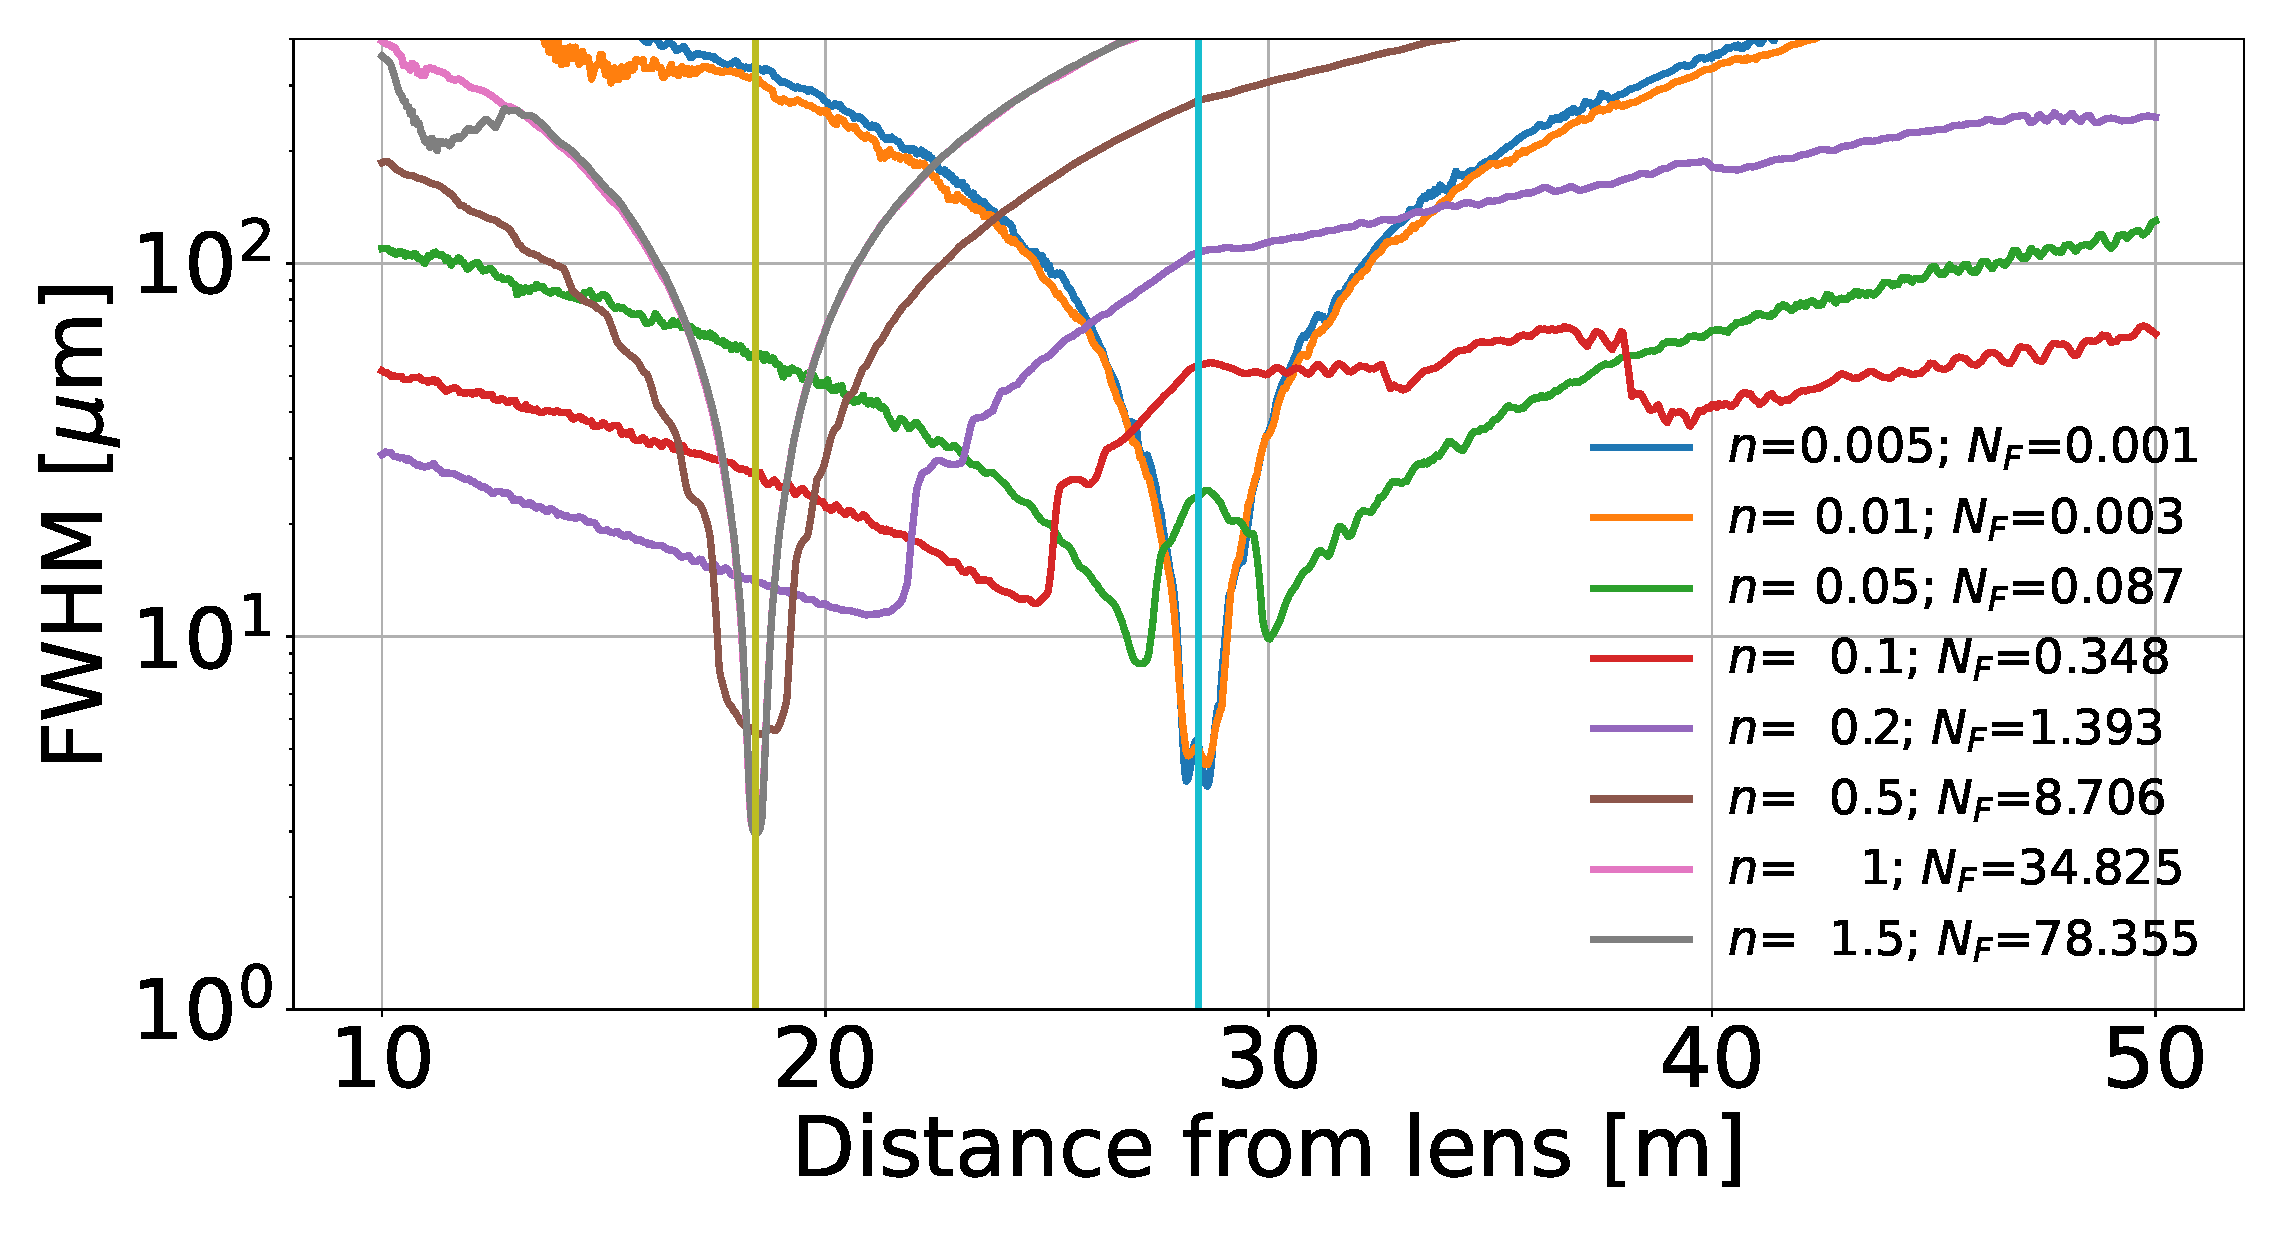
\includegraphics[width=0.95\textwidth]{figures/oneTF_UndSource_RectSlit_R200um.eps}
    %     \includegraphics[width=0.95\textwidth]{figures/oneTFundGSM_200um.eps}
    % \includegraphics[width=0.95\textwidth]{figures/oneTFundHYBRID_200um.eps}
    % \includegraphics[width=0.95\textwidth]{figures/oneTFund_100um.png}

    \caption{Evolution of the size of a coherent undulator beam cropped by a slit and focused by a lens of $R$=~\SI{0.2}{\milli\meter} 
    The plot shows the FWHM of the beam  as a function of the distance from the lens. The aperture is open at $a = n \times a_{FWHM}$ with different values of $n$ (shown in the legend) and $a_{FWHM}$=\SI{565}{\micro\meter} (the beam FWHM at the aperture plane). The focal positions given by geometrical optics are represented for the source placed wither at the ID position (yellow vertical line) or at the slit position (blue vertical line).
    The Fresnel number $N$ calculated at the slit plane is also marked in the legend.
    }
\end{figure}

Fig.~\ref{fig:oneTFund} shows the evolution of the beam after being focused by the lens. With the open slit the geometrical optics give a focal position $q=$~\SI{18.4168}{\meter} (source at the ID position, distant $p$ from the lens) and $q_a=$~\SI{28.4089}{\meter} (source at slit position, distant $p_a$ from lens). It can be noticed that for $n\ge$1 (Fresnel number $N\ge$35) the situation does not change with respect the open slit because the cropping by the slit is negligible. For $n=0.5$ ($N=8.7$, brown line) the FWHM of the focal size increases and the depth of focus also increases, manifested in a flat depression. For smaller values of $n$ and $N$ the minumum shifts to higher distances (e.g., $n=0.1$ red line) and becomes less pronounced. For $n$=0.05 (green line), a small beam size is found again close to the $q_a$ position, but it presents twin minimum due to the effect of the interference fringes in the intensity distribution. Both minima converge to a the $q_a$ position for $n\le$~0.01 (orange line). 

When the focal distance of the lens is reduced (using lenses with smaller radius, or piling several lenses), the $q$ and $q_a$ positions shift to shorter distances,
%(instead of longer distances as sound in Fig.~\ref{fig:oneTFund}), as found for instance in \cite{westfahl},
and  $|q-q_a|$ also reduces. They converge to a single position: the lens focal length $q=q_a=F$. This happens when both source-lens and slit-lens distances can be considered at infinite. 

The dimension of the waist can be calculated using geometrical concepts only for the limiting cases of waist at $q$ and $q_a$. Here, for the waist at $q$, the beam size is the source size times the magnification (distance lens-waist over distance lens-source) and for the waist at $q_a$, the beam size is the slit aperture times the magnification (distance lens-waist over distance slit-lens). This has been verified numerically (not shown). However, for intermediate slit apertures, where the waist position is in between $q$ and $q_a$, the waist size is different to that predicted by geometric optics.
Indeed, it can be observed in Fig.~\ref{fig:oneTFund} that for these intermediate slit apertures that crop the beam, the waist size is larger than those found at limiting positions $p$ and $p_a$.
This is an important fact: A good focusing, i.e., a very small beam size is only obtained in the limiting cases of open slit and almost-closed slit. This means that for a fully coherent beam, the slit disturbs the focusing and should be avoided. The diffraction at the slit creates an an spurious divergence that affects the lens power. 

\todo{MOVE TO DISCUSSION? This degradation of the focal dimension when focal position cannot be predicted by the geometrical optics adds difficulty to the design of optical systems: the slit must be closed enough to guarantee a good coherence, but opened enough to maintain the focal position not far from that of the geometrical optics.} 


The calculation shown in Figure~\ref{fig:oneTFund} refers for the zero emittance case (complete coherence, or $CF_h=CF_v=1$). Next section extends these results to the more realistic case of finite emittance.

\subsubsection{Partial coherence} The mission of the slit is to improve beam coherence (increase coherent fraction). In storage rings like ESRF-1, with $CF<10^{-3}$, the slit must be almost closed to gain coherence, thus forming a secondary source. For storage rings like EBS, with $CF > 10^{-2}$, the selection of the slit aperture $a$ is crucial: the slit must be closed until the the desired $CF$ is obtained, but not more, because it not only reduces intensity but also deteriorates the focusing. 

\begin{figure}
    \centering
    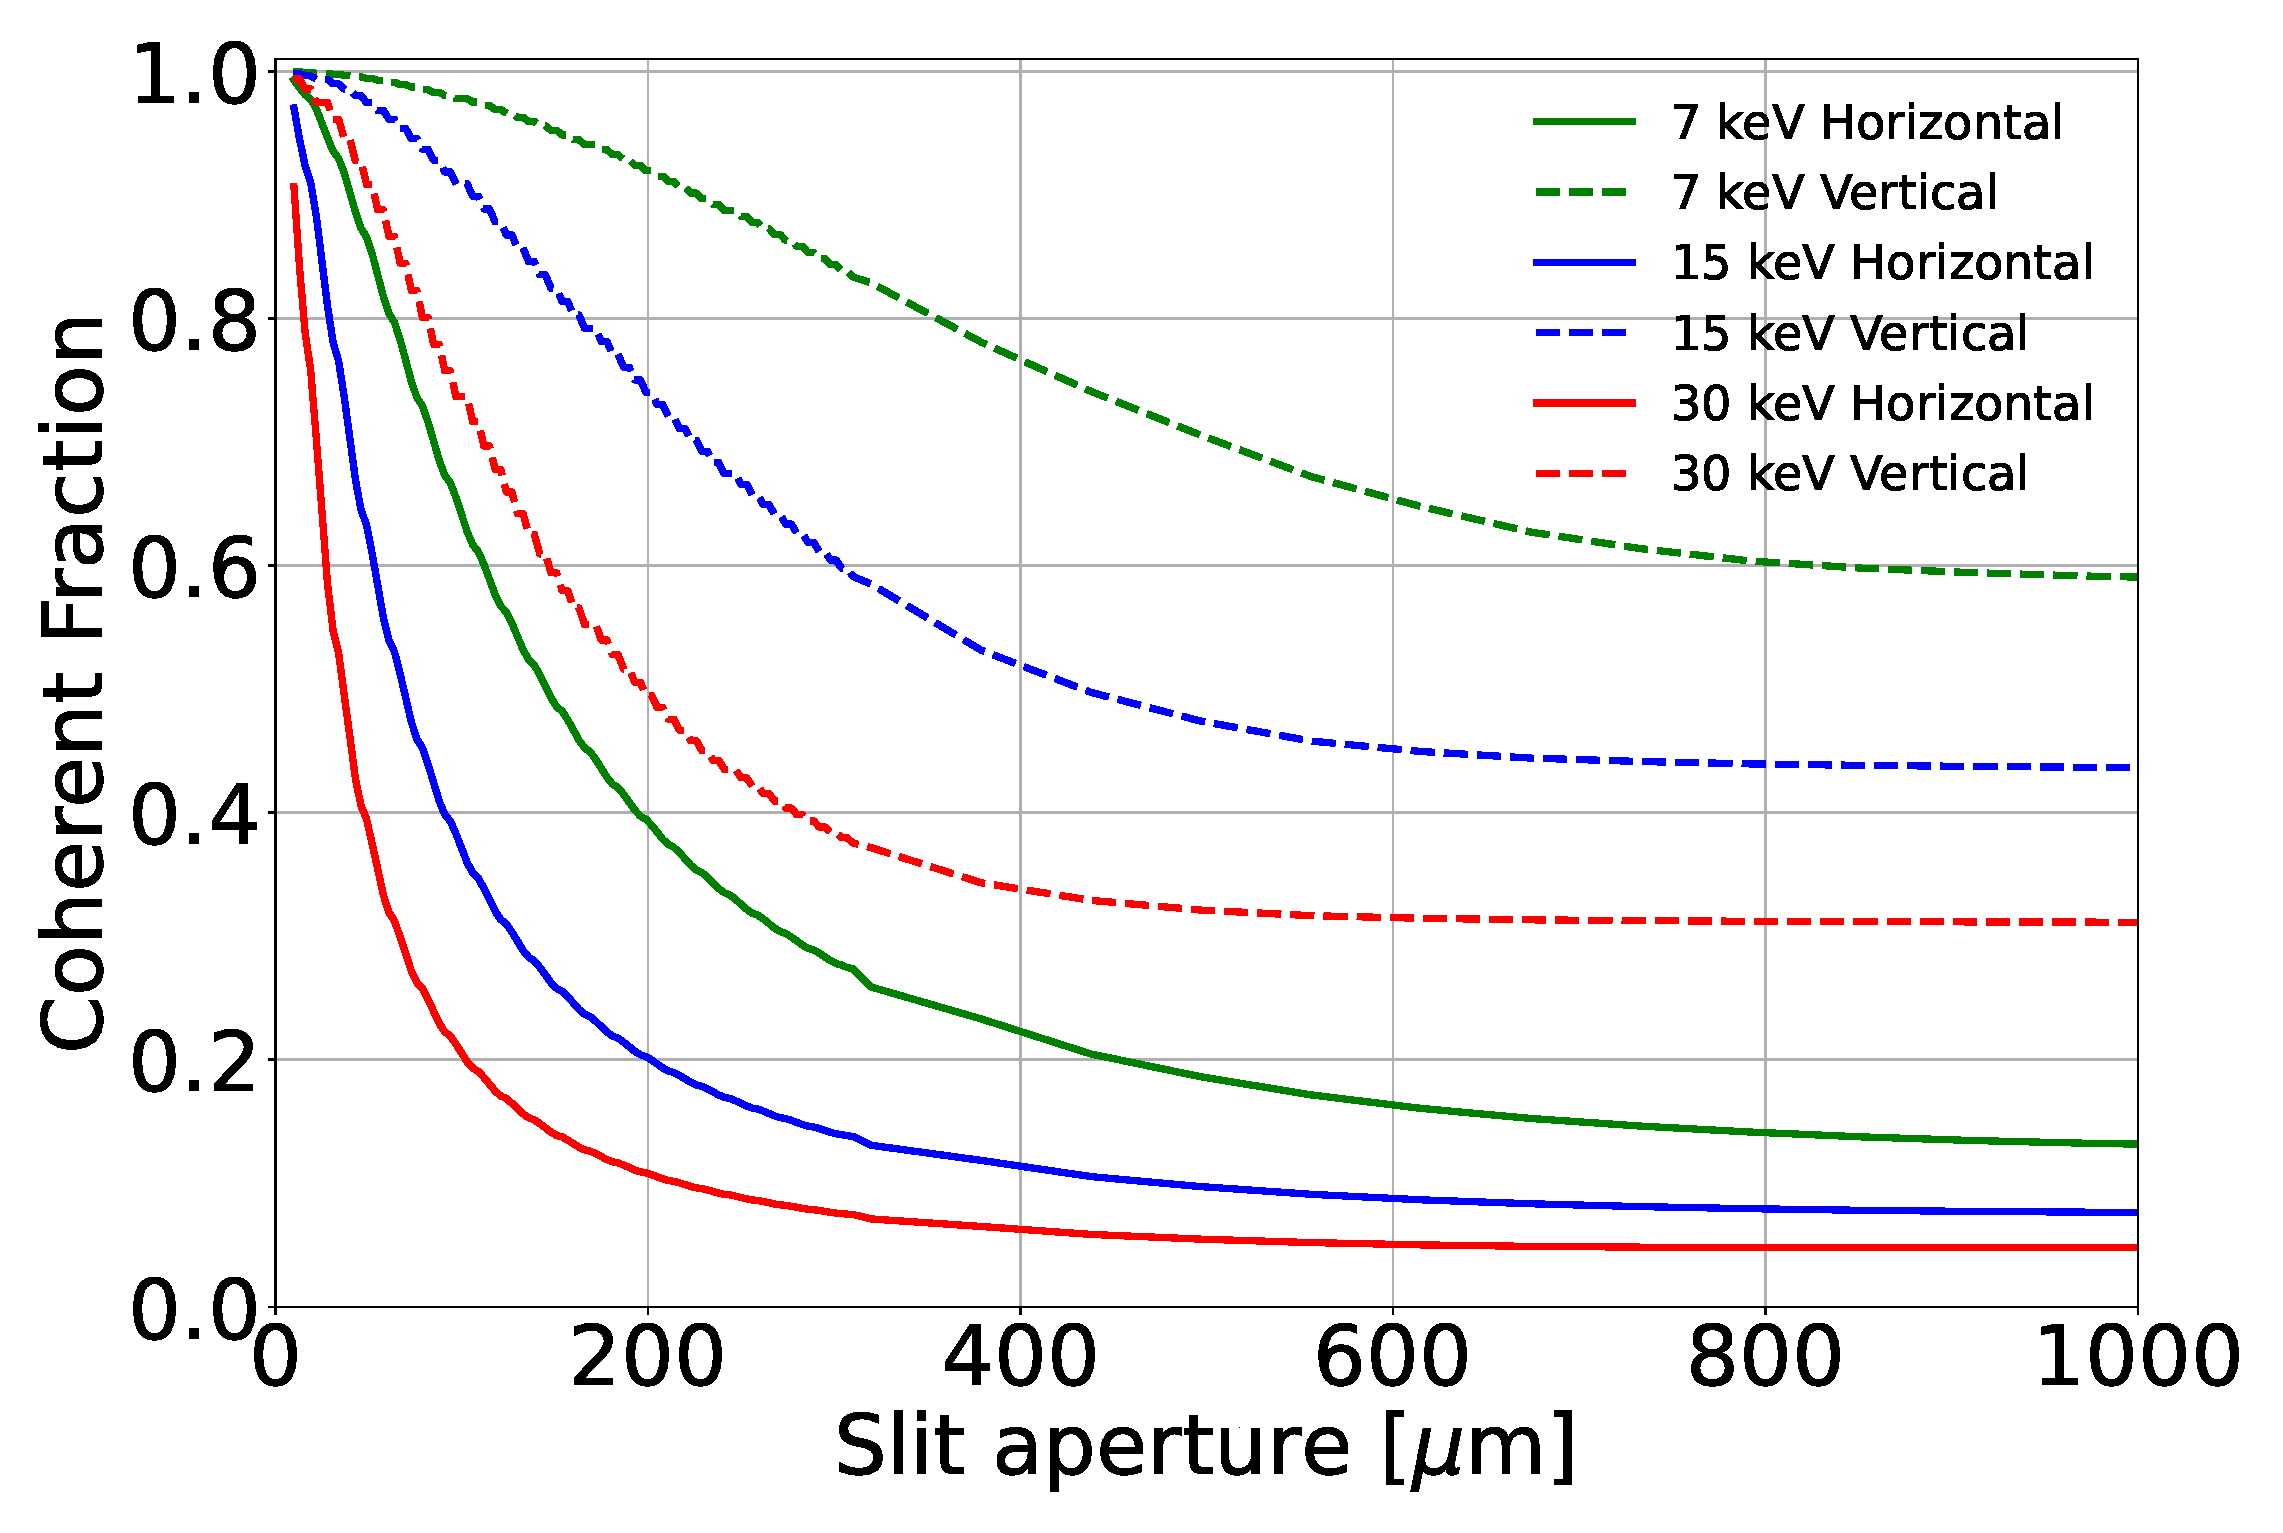
\includegraphics[width=0.95\textwidth]{figures/cf_vs_aperture.eps}

    \caption{
    Coherent fraction in the horizontal and vertical directions for different photon energies as a function of the slit aperture $a$. The slit is placed at \SI{36}{\meter} from the ID. 
    % Top axis shows the $n$ factor as in Fig.~\ref{fig:oneTFund} ($n=565/a$).
    }
    \label{fig:cf_vs_aperture}
\end{figure}

We used the EBS-ESRF emittance values\footnote{We used over this work the following values of electron beam sizes at the center of the straight section: $\sigma_x=~\SI{29.7}{\micro\meter}$,
$\sigma_{x'}=~\SI{4.37}{\micro\radian}$,
$\sigma_y=~\SI{5.29}{\micro\meter}$,
$\sigma_{y'}=~\SI{1.89}{\micro\radian}$, corresponding to beam emittances:  $\epsilon_x=~\SI{130}{\pico\meter \radian}$,
$\epsilon_y=~\SI{10}{\pico\meter \radian}$, and beta functions
$\beta_x=~\SI{6.8}{\meter}$,
$\beta_y=~\SI{2.8}{\meter}$
},
to perform a coherent mode decomposition of the undulator source. This is required to include the partial coherent effects. This is done for the horizontal and vertical directions, resulting a coherent fraction (at 7 keV) of $CF_h=$13\% and $CF_v=$58\%, respectively. These values are much higher than for the old ESRF-1 source, but still low to justify approximating the beam by a coherent beam. Therefore, we propagated a number of modes large enough to contain more than 99\% of the source intensity (36 modes in H and 8 in V). The illumination at the entrance slit plane is \SI{610}{\micro\meter} in H times \SI{566}{\micro\meter} in V. The slit aperture is used to tune the coherence of the beam: closing the slit reduces the $CF$. In the limit (zero aperture) the beam after the slit is fully coherent ($CF=1$), but obviously with zero intensity. The choice of the right slit aperture comes from a compromise between coherence and flux. The Figure~\ref{fig:cf_vs_aperture} shows the $CF$ after of the H and V 1D beams after the slit for different slit apertures. From this figure we select the apertures to be used in the following simulations. We selected at 7 keV photon energy a first $CF_h=CF_v=$90\% in both horizontal and vertical (thus with a combined 2D  $CF=CF_h CF_v=$81\%) obtained with slit apertures of
$a_h$=~\SI{40.3}{\micro\meter}, and 
$a_v$=~\SI{227}{\micro\meter} (horizontal and vertical, respectively), and a second $CF_h=CF_v=$70\% (thus 2D $CF$ of about 50\%), with 
$a_h$=~\SI{85.1}{\milli\meter}, and 
$a_v$=~\SI{506.7}{\milli\meter}. The case of the ``open" slit that does not crop the beam is also included (this is obtained, for example, with $a_h$=~\SI{1}{\milli\meter} and $a_v$=~\SI{1.5}{\milli\meter}).

%For energy  7 keV, and CF: 0.9 I need slit  40.3 X 227.0 um2
%For energy  7 keV, and CF: 0.7 I need slit  85.1 X 506.7 um2
%

\begin{figure}\label{fig:oneTFundPartialCoherence}
    \flushleft a) {\it horizontal}\\ \centering
    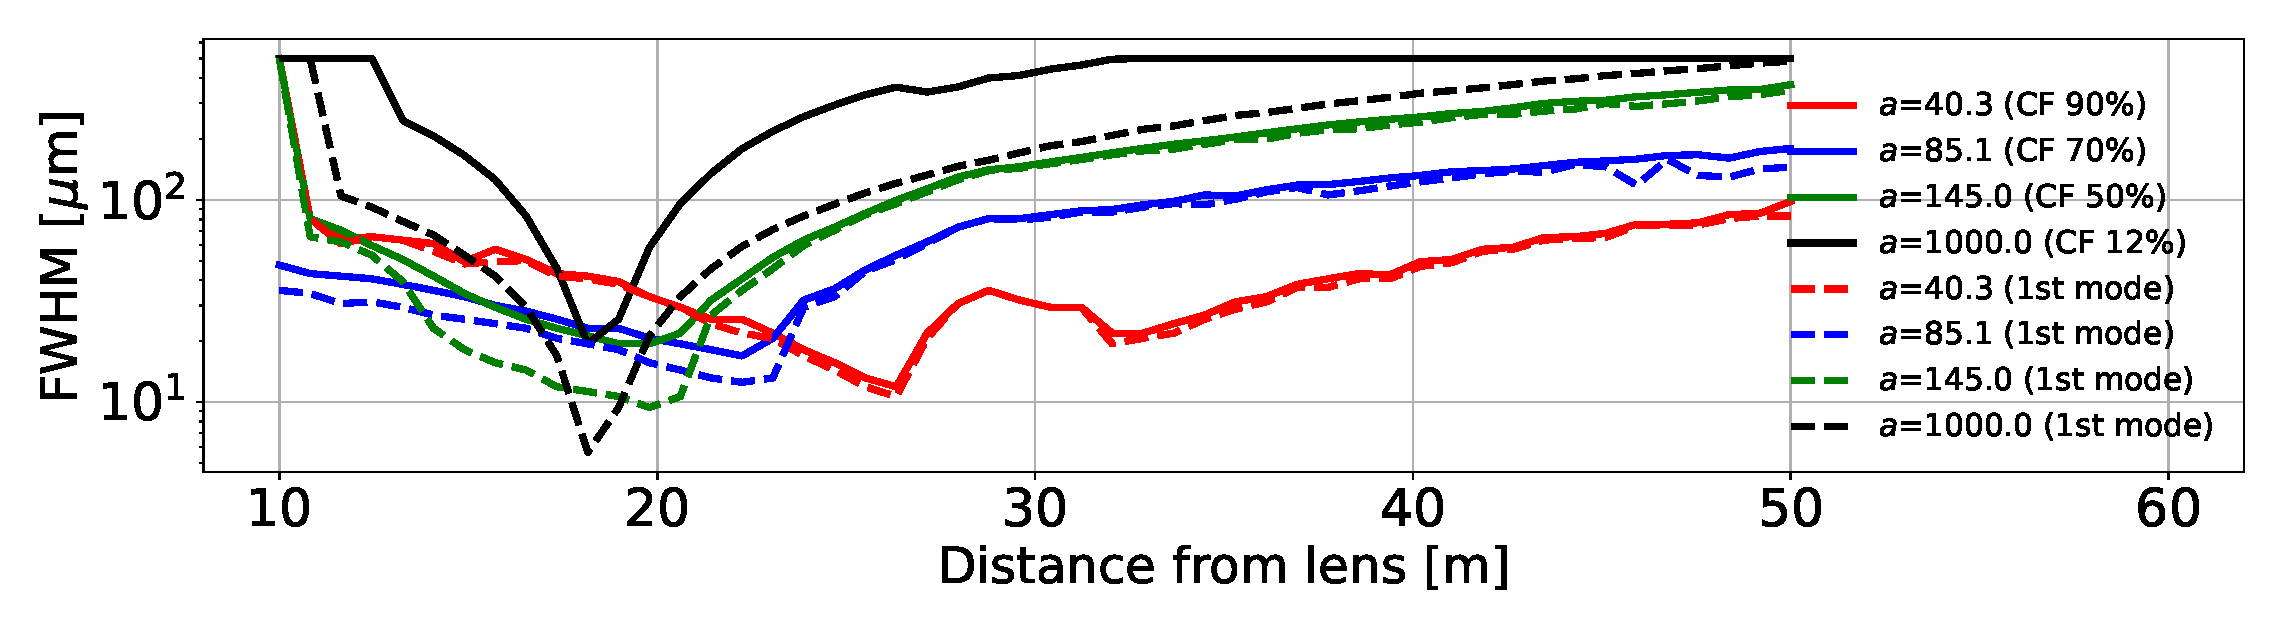
\includegraphics[width=0.95\textwidth]{figures/oneTF_UndSource_RectSlit_R200um_PartialCoherence_h.eps}
    \flushleft b) {\it vertical}\\ \centering
    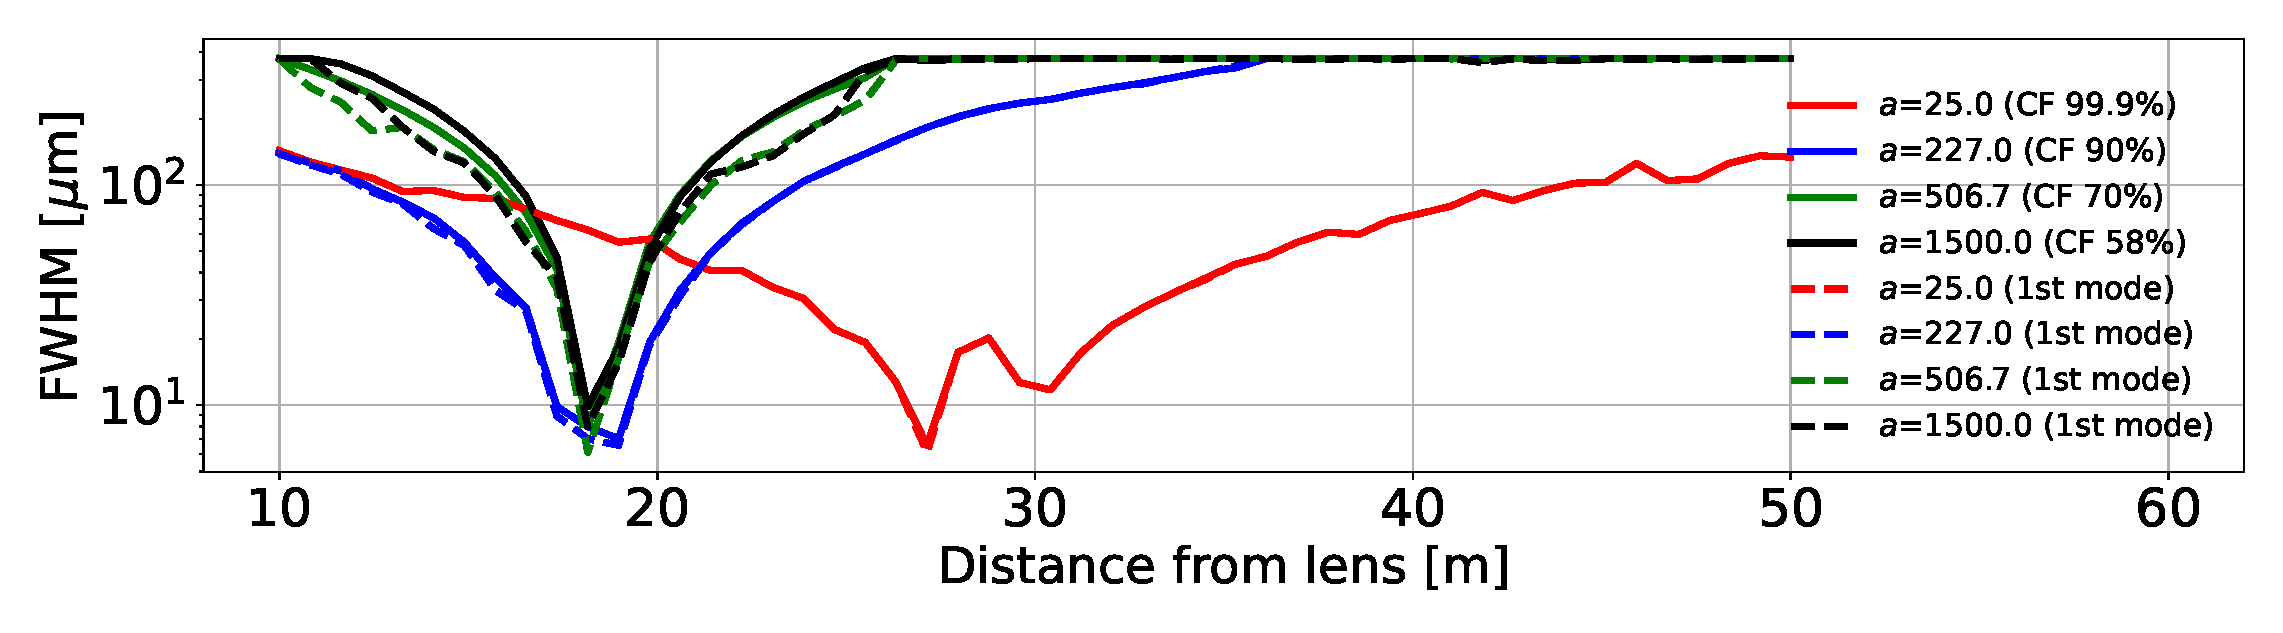
\includegraphics[width=0.95\textwidth]{figures/oneTF_UndSource_RectSlit_R200um_PartialCoherence_v.eps}

    \caption{Evolution of the size of a coherent undulator beam cropped by a slit and focused by a lens of $R$=~\SI{0.2}{\milli\meter} in the a) horizontal and b) vertical directions.
    The plot shows the FWHM of the beam  as a function of the distance from the lens.
    Full lines correcpond to the partial coherent (multimode) beam, whereas the dashed lines correspond to the full coherent beam (first mode). Different slit apertures are used for obtaining different coherent fraction after the slits (marked in legend).
    }
\end{figure}

Figure~\ref{fig:oneTFundPartialCoherence} shows the focal size along the optical axis for these apertures in the horizontal and vertical planes. We have calculated the case of the partially coherent beam (multi-mode) with the case of fully coherent beam (only the first coherent mode). We observe that the focal positions (the minima of the plot lines) do not change significantly when comparing the partially coherent and the full coherent beam. However, the focal dimension changes significatively in the case of low coherence (e.g., in the cases $CF_h\le$70\%). In the vertical, where the source much more coherent (58\%) there is no differences in sized when going from partial to fully coherent beams. Looking to the focal position shift versus sllit aperture we find important differences in the horizontal and vertical. In the horizontal, the cropping of the beam by the slit is important as we need to increase the $CF_h$ from the source (13\%) to values required by the experiments, usually larger than 50\%. This produces a gradual shift of the focal position from the position of the geometrical image of the ID source (black line in panel a)) to the geometrical image of the slit (red line in panel a)). However, in the vertical plane, the slit crops the beam only slightly, and closing the slit to go from the source $CF_v$=58\% to values up to 90\% do not produce any focal shift from the  position of the geometrical image of the ID source. Only when the slit is very much closed (e.g., $a_v$=~\SI{25}{\micro\meter}, red curve) the focal position shifts to the geometrical image of the slit. This case is in principle not interesting experimentally as it reduces the intensity from an already quite coherent beam ($CF_v$=90\%). 

In this section, we have supposed that the 2D beam can be separated in two 1D beams, for H and V directions. No other approximations were made: we used the full undulator source, performed coherent mode decomposition, used an aperture with a rectangular function, and used a Be lens with the real parabolic profile (with thickness $t=$~\SI{50}{\micro\meter} and aperture \SI{1}{\milli\meter}). Some of these factors could be relaxed, for example using slits with absorption by Gaussians, and ideal lenses. In Appendix \ref{appendix:comparison} we have studied the resulting beam evolution considering these approximations. We also noticed that ray-tracing using the hybrid method \cite{codeHYBRID} give similar results (this will be discussed in section \ref{sec:discussion}). 

\section{Pairing two transfocators}

%http://lpc1.clpccd.cc.ca.us/lpc/molander/PDFs/Twolenses.pdf

We study here an optical system composed by two lenses (of focal lengths $f_1$ and $f_2$) separated by a distance $D$. Following \cite{Goodman85}, the relationship between object-to-lens-1 distance $p_1$ and the lens-2-to-image distance $q_2$ positions is
\begin{equation}
\label{eq:twolens}
    D-(f_1+f_2)=\frac{f_1^2}{p_1-f_1} + \frac{f_2^2}{q_2-f_2}
\end{equation}

The global magnification is the product of the magnification of the individual lenses. It can be written as

\begin{equation}
\label{eq:magnification}
    M=M_1 M_2=\frac{1-q_2/f_2}{1-p_1/f_1}
\end{equation}

The magnification is not dependent on $D$, however the length of the optical system $L=p_1+D+q_2$ will change if one changes the focal distances of the lenses. For a constant $L$ one can change magnification by changing the inter-lenses distance $D$ (zoom effect). In a synchrotron beamline using transfocators, the magnification can be changed by varying the focal lengths of the transfocators (by adding or removing individual or group of lenses in the transfocator).

We analyze here how to design an optical system using two transfocators and how to set it for the desired focal size or magnification. We start using the oversimplified assumptions of geometrical optics, for then using wave optics simulations to include diffraction effects with a fully coherent beam, and lastly we analyse the focusing system when it is illuminated by a partial coherent beam.

\begin{table}[]
    \label{table:id18parameters}
    \caption{Position of the two transfocators, slit and sample (focal point) corresponding to the ID18 beamline configuration under study. }
    \centering
    \begin{tabular}{l|c|c}
         element & position [m] & comment\\
         ID (undulator) source& 0 & U18 $N_u$=138 $K$=1.185 (7 keV)\\
         Slit & 36 &
         variable aperture $a_h\times a_v$
         \\
         Transfocator 2D & 65 & 
         %$f_H=58.7; f_V=54.3$ 
         \\
         Transfocator 2D & 170 & $D$=~\SI{105}{\meter} \\
        %  Transfocator 2D & 170 & position 1 {\bf FO1}, $D$=~\SI{105}{\meter} \\
        %  Transfocator 2D & 192 & position 2 {\bf FO2}, $D$=~\SI{127}{\meter}  \\
         sample & 200 & focal plane
    \end{tabular}


\end{table}

The system under analysis contains two transfocators, idealized as two real lenses of variable curvature radius. A slit of aperture $a_h$ in H and $a_v$ in V is placed upstream the lens one. The positions of the elements is determined by room constraints and are considered fixed (although different values could be studied). We set the distances matching the requirements of the EBS-ESRF ID18 beamline (see Table~\ref{table:id18parameters}), and we analyzed the system at a photon energy of 7 keV. We study the variation of the spot size as a function of the focal distances. The final goal would be set the transfocators focal lengths (obtained by a particular combination of lenses) to get the desired focal size. 

% For the practical purposes of ID18 (see parameters in Table~\ref{table:id18parameters}), we study two possible positions of lens 2: at \SI{164}{\meter} from the source (initial design, $D$~= \SI{99}{\meter}) and at \SI{188}{\meter} from the source ($D$~= \SI{123}{\meter}). The later implies a shorter, thus cheaper, experimental hutch. 

% Because the effect of shift of focal position due to slit diffraction, discussed before, we consider the two geometrical limiting cases: i) the source at its real position, and ii) the source at the slit position (limit of ``very closed slit"). We expect that the real case will lie in between these two extremes. 



\begin{figure}\label{fig:f1f2map}
    \centering
    % \includegraphics[width=0.95\textwidth]{figures/Figure_trajectories_99.png}
    % \includegraphics[width=0.95\textwidth]{figures/Figure_trajectories_123.png}
    
    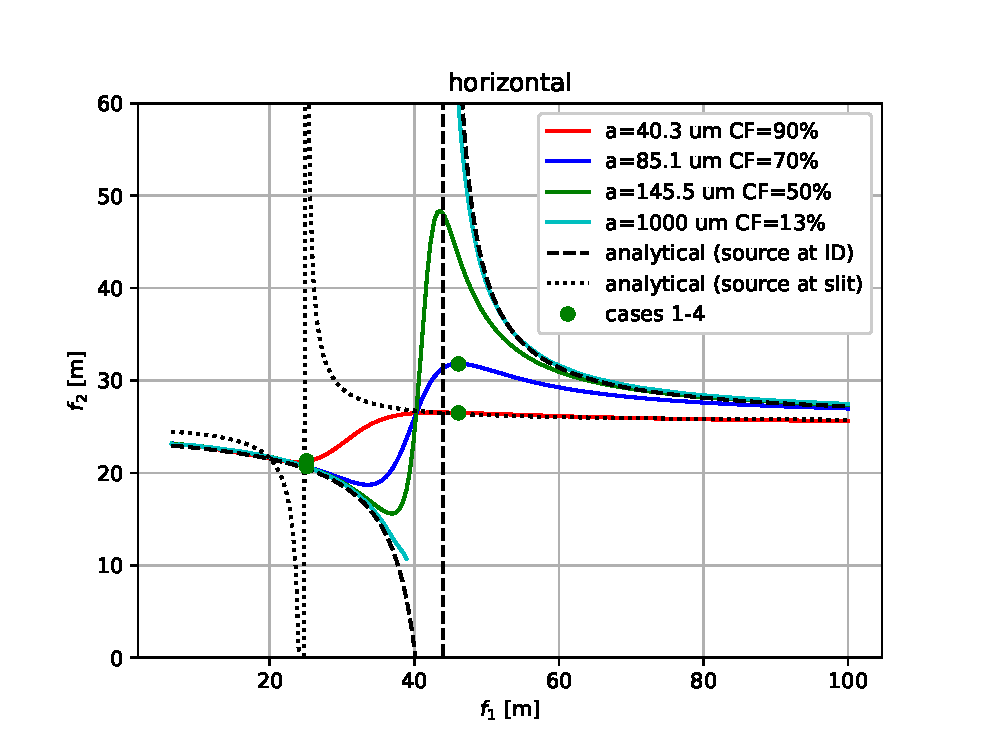
\includegraphics[width=0.95\textwidth]{figures/f1f2_h.eps}
    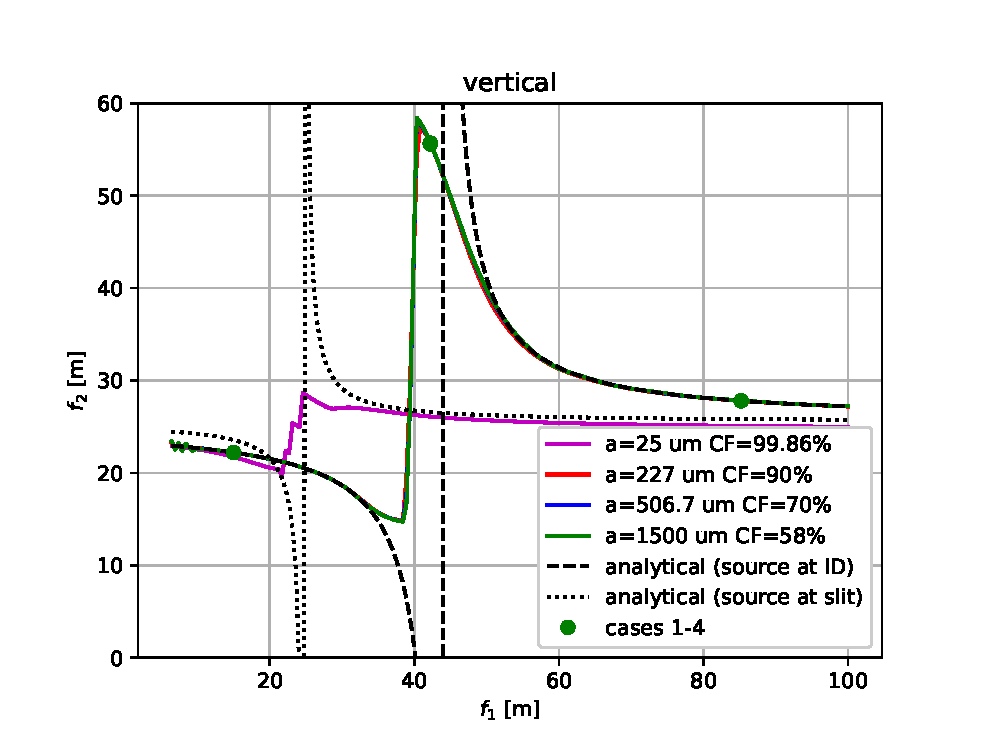
\includegraphics[width=0.95\textwidth]{figures/f1f2_v.eps}

    \caption{Trajectories $(f_1,f_2)$ for $D$~= \SI{105}{\meter} calculated numerically for different values of apertures. Panel a) is for the horizontal direction and panel b) for the vertical. 
    % (\inred{top panel}) and $D$~= \SI{123}{\meter} (\inblue{bottom panel}).
    Analytical values displayed are obtained using equation~\ref{eq:twolens} with $p_1$~= \SI{65}{\meter} (object at source position) (solid lines) or $p_1$~= \SI{30}{\meter} (object at slit position) (dashed lines). 
    }
\end{figure}

For fixed distances $p_1$, $D$ and $q_2$, and also a given value of $f_1$, one can calculate analytically $f_2$ using  equation~(\ref{eq:twolens}) and the corresponding magnification $M$ in the framework of geometrical optics. Taking $f_1$ as variable parameter,  
% Fig.~\ref{fig:f1f2map} shows the maps $f_1$, $f_2$ for two values of $D$.
Fig.~\ref{fig:f1f2map} shows the trajectories of $f_2$ as a function of a variable $f_1$. 
The choice of one pair $(f_1,f_2)$ from these curves guarantees that the focus is at the sample position ($L=p_1+D+q_2$~= \SI{200}{\meter} from source).

Figure~\ref{fig:f1f2map} also shows the value of $f_2$ optimized numerically\footnote{Calculations in this section use a Gaussian window to model slit aperture to minimize diffraction fringes}. They are calculated from the analysis of the wavefront phase impinging on lens 2. A correction profile to focus on the sample is calculated using the method described in section~\ref{sec:refractorCorrector}. This profile is fitted with a circle over the central part of the lens, thus giving the radius of curvature or the most adequate lens, and also the its focal length. 
The $(f_1,f_2)$ curves depend strongly on the slit aperture in the horizontal, because of the low $CF_h$ of the source (12\%) is highly increased by the slit. In the vertical the source is more coherent ($CF_v$=58\%) therefore the slit improves the $CF_v$  and there is not much change in the trajectories up to values of 90\%. However, in the case of a slit with $a_v$=~\SI{25}{\micro\meter} that is acting as a pinhole the trajectories (red line) approaches the results of the geometrical optics considering the source at the slit position. 
% It can be observed that the value of $f_2$ obtained numerically goes from the first branch of the analytical values (when the object it at the source position) to  the second branch (when object is at slit), as common sense anticipated. 

\begin{figure}
    \centering
    % \includegraphics[width=0.95\textwidth]{figures/Figure_magnification_99.png}
    %\includegraphics[width=0.95\textwidth]{figures/Figure_magnification_123.png}
    
    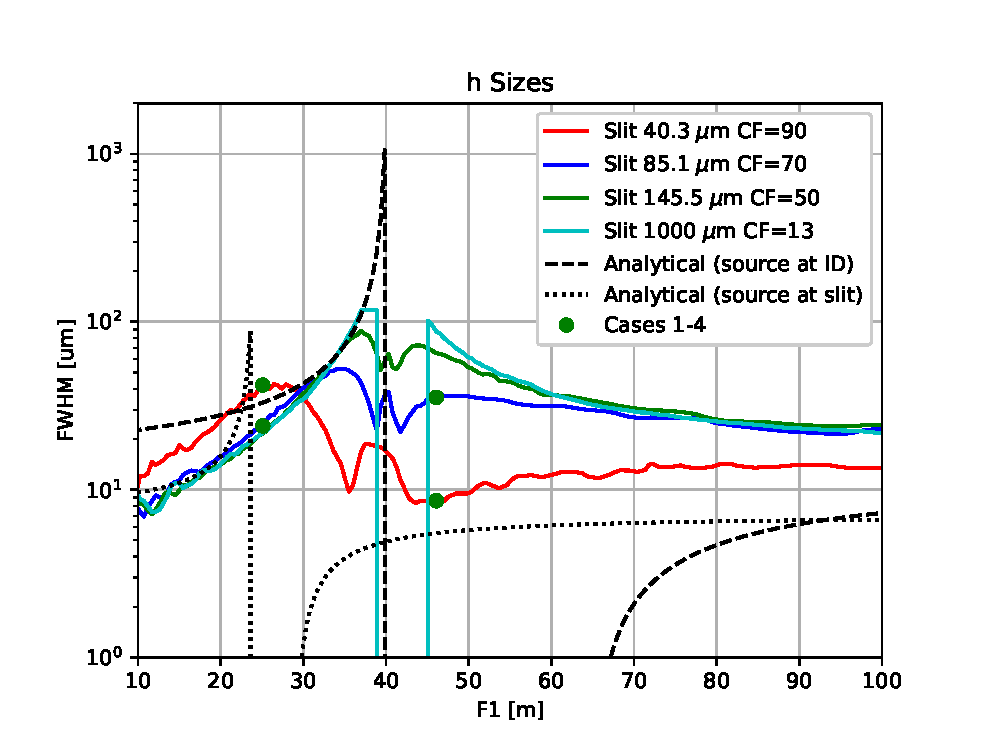
\includegraphics[width=0.95\textwidth]{figures/sizes_h.eps}
    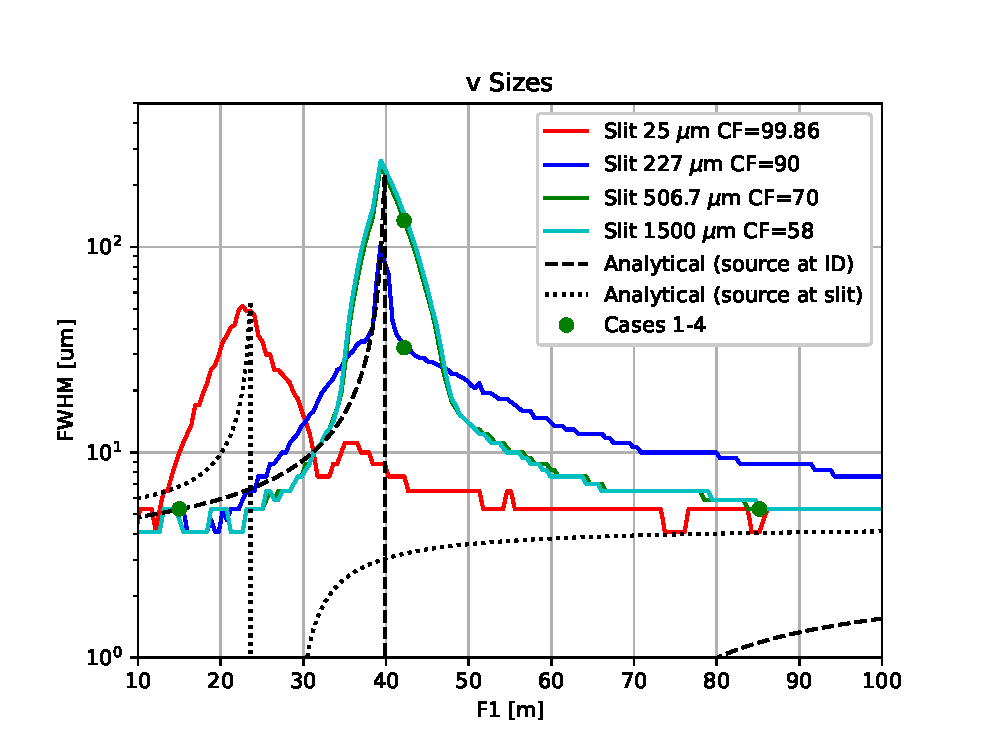
\includegraphics[width=0.95\textwidth]{figures/sizes_v.eps}
        
    \caption{Focal sizes obtained by a two transfocator system as a function of focal length of lens 1 $f_1$. The focal length $f_2$ of the second lens is obtained from the trajectories in Fig.~\ref{fig:f1f2map}. 
    Analytical values are obtained using equation~(\ref{eq:magnification}) with $p_1$~= \SI{65}{\meter} (object at source position) (solid lines) or $p_1$~= \SI{29}{\meter} (object at slit position) (dashed lines). 
    % Numerical values \ingreen{green} are obtained for the slit (upstream lens 1) either open or closed to $a$~= \SI{25}{\micro\meter}.
    }
    \label{fig:focalSizes}
\end{figure}

Figure ~\ref{fig:focalSizes} shows the calculated focal sizes. Analytical values based on geometrical optics use  equation~(\ref{eq:magnification}). It can be observed the limited applicability of the analytical values, thus the necessity of performing the numerical simulations to get accurate values of beam sizes. In the horizontal, for slit apertures $a_h>$~\SI{40}{\micro\meter} the sizes change considerably for different $a$ values. The focusing characteristics of the system depends highly on the diffraction effects produced at the slit. For the slit $a_h$=~\SI{40.3}{\micro\meter} ($CF_h=$90\%) the focal size can vary from roughly 10 to 50 microns.  In vertical the focal size can be changed from 5 to 100 \SI{}{\micro\meter} at at $CF_v=$90\%.

% The numerical values are calculated in two cases. First with the open slit, a case that would correspond to the analytical case with object at the source position. This is verified in the top panel for $f_1>30$. Second with a slit closed to $a$~= \SI{25}{\micro\meter} which should approach the analytical results when the object it at the slit position. 

% \inblue{A conclusion from this graphic is geometric magnification could only be used to calculate focal size only in the case of open slit. When the slit crops the beam, numerical calculations are needed.}

% \todo{redo these figures and discussion.}






% To simulate a more realistic case, we included partial coherence. Fig.~\ref{fig:sizes} displays the image sizes in the case of coherent source (first coherence mode) and partial coherent source (using 50 coherent modes to mimic the undulator in horizontal).
% The most realistic case is the partial coherence case for the \SI{25}{\micro\meter} slit. From the graphics (orange dash-dotted lines) it can be seen that for $D=$~\SI{99}{\meter} (FO1) we obtained a focal spot between 15-35 \SI{}{\micro\meter} \inblue{(11.8-21.6 calculated by Marco)}; and 1.5-10 \SI{}{\micro\meter} \inblue{(15.4-5.3??? calculated by Marco, FO2)} for $D=$~\SI{123}{\meter}.  



% \begin{figure}
%     \centering
%     \includegraphics[width=0.95\textwidth]{figures/Figure_sizes_99.png}
%     \includegraphics[width=0.95\textwidth]{figures/Figure_sizes_123.png}
%     \caption{Beam sizes at the image position (spot at sample) for a two transfocator system as a function of focal length of lens 1 $f_1$. The lens 2 focal $f_2$ comes from the trajectories in Fig.~\ref{fig:f1f2map}.
%     Top panel is calculated for \inred{$D$~= \SI{99}{\meter}} and bottom panel with \inblue{$D$~= \SI{123}{\meter}}.
%     Numerical values are obtained for the slit (upstream lens 1) either open (solid lines) or closed to $a$~= \SI{25}{\micro\meter} (dash-dotted lines). Simulations are done for a \ingreen{coherent source (green lines)} (\SI{15.14}{\micro\meter} FWHM) and partial coherent source (orange lines) (\SI{71.35}{\micro\meter} FWHM).
%     }
%     \label{fig:sizes}
% \end{figure}


% Some numerical values are in Table~\ref{table:comparison}.
% \begin{table}[]
%     \caption{Simulations}
%     % \label{tab:my_label}
%     \centering
%     \begin{tabular}{ccc}
%          $f_2$ [m] & This work & Marco \\
%         \hline
%          39.7  & 37.00  & 21.5  \\
%          29.38 & 32.19  &   \\
%     \end{tabular}
%     \label{table:comparison}
% \end{table}

     % Appendices appear after the main body of the text. They are prefixed by
     % a single \appendix declaration, and are then structured just like the
     % body text.

\section{Simulations of the complete beamline}

In this section we analyse in detail the full beamline using several methodologies. We analyze in detail the intensity distribution at the focal plane for four cases. They have been selected from the results in Fig.~\ref{fig:focalSizes}). The first case is selected to obtain a small spot (about \SI{5}{\micro\meter}) and the second one a large spot (more than \SI{30}{\micro\meter}).  For these cases the slits are selected to match a $CF_h=CF_v=$90\% for a photon energy of \SI{7}{keV}. The values are shown in Table~\ref{table:2Dusercases}. The cases 3 and 4 follow the same logic but the slits are opened to obtain a less coherent beam ($CF_h=CF_v=$70\%). The analysis is made with different methodologies, using different software codes, following an hierarchical approach, as discussed in \cite{hierarchical}, with the idea to evaluate accuracy and computational effort, and select the most advantageous method for the analyzed problem. This multi-method analysis will also validate the new method introduced in this work, the 1D CMD, by comparing its results with other well-known simulation tools. 

\begin{table}[]
    \label{table:2Dusercases}
    \caption{Configurations selected for 2D simulations. Slit aperture $a$ is selected for obtaining $CF_h=CF_v=$90\% in cases 1 and 2, and $CF_h=CF_v=$70\% in cases 3 and 4. Data is obtained from Fig.~\ref{fig:focalSizes}.
    }
    \centering
    \begin{tabular}{c|c|c|c|c|c|c|c}
         case h/v & $a$ [\SI{}{\micro\meter}] & $f_1$ [m] & $f_2$ [m] & $R_1$ [\SI{}{\micro\meter}]& $R_2$ [\SI{}{\micro\meter}] & size [\SI{}{\micro\meter}]& index\\
         \hline
1 h &      40.3 & 46.1 &     26.5 &     641.9 &     369.5 &     8.6 &     86 \\
1 v &      227.0 & 15.0 &     22.2 &     209.4 &     309.6 &     5.3 &     21 \\
\hline
2 h &      40.3 & 25.1 &     21.3 &     349.1 &     296.3 &     42.0 &     42 \\
2 v &      227.0 & 42.2 &     55.6 &     588.6 &     775.3 &     32.3 &     78 \\
\hline \hline
3 h &      85.1 & 46.1 &     31.8 &     641.9 &     443.7 &     35.5 &     86 \\
3 v &      506.7 & 85.2 &     27.8 &     1187.4 &     387.6  &     5.3 &     168 \\
\hline
4 h &      85.1 & 25.1 &     20.7 &     349.1 &     288.7 &     24.0 &     42 \\
4 v &      506.7 & 42.2 &     55.7 &     588.6 &     776.0 &     134.3 &     78 \\

    \end{tabular}
\end{table}

\begin{table}[]
    \label{table:comparison}
    \caption{Comparison of sizes (FWHM, in \SI{}{\micro\meter}) calculated with different methods for the cases defined in Table~\ref{table:2Dusercases}.
    In brackets, the values for the fully coherent beam (single electron with SRW, first coherent mode with COMSYL/WOFRY), and zero emittance with Hybrid).
    Coherent fraction is square brackets \inblue{[CF]}}
    \centering
    \begin{tabular}{p{0.05\textwidth}|c|c|c|c|c|}
         case h/v &
         Wofry1D&
         COMSYL&
         SRW&
         Hybrid \\
         \hline
1 h  & 8.6,8.5(8.1) \inblue{[94]}  & 10.0 (9.9)  & 8.6 (7.5)   & 17.3 \\
1 v  & 5.3,4.8(4.8) \inblue{[97]}   & 4.7 (5.1)   & 4.6 (4.6)   & 3.3 \\
\hline
2 h  & 42.0,39.9(38.2) \inblue{[94]} & 39.5 (39.5) & 40.0 (36.1)  & 39.9 \\
2 v  & 32.3,32.4(29.6) \inblue{[90]} & 30.6 (29.3) & 34.4 (29.6)  & 74.0 \\
\hline
3 h  & 35.6,37.5(29.0) \inblue{[77]} & 36.6 (28.1) & 40.3 (28.4)  & 43.3 \\
3 v  & 5.3,6.1 (4.9)  \inblue{[77]} & 6.4 (5.7) & 6.3 (4.6)   & 6.5 \\
\hline
4 h  & 24.0,24.6(19.1)\inblue{[77]}  & 26.1 (18.6) & 27.4 (18.0)  & 27.1 \\
4 v  & 134.4,133.7(110.3)\inblue{[71]}& 111.7 (90.4) & 137.4 (132.0) & 150.2 \\
    \end{tabular}
\end{table}


\subsection{Model WOFRY 1D}
We have recalculated with Wofry 1D the cases shown in Table~\ref{table:2Dusercases}. We then combined the 1D horizontal and vertical profiles (using the outer product) to form the 2D intensity profile at the focal plane. Results are shown in Fig.~\ref{fig:2DWofry1D}. Looking at the intensity distributions, it can be observed a variety of features that are due to the diffraction effects. Case 1 shows an horizontal profile mostly triangular with shoulders that evidence small diffraction fringes. The fringes are more resolved in the vertical direction. Case 2 horizontal presents a soft Gaussian-like profile, but in vertical important symmetric shoulders are appreciated. Case 3 shows a smooth Gaussian profile in horizontal \todo{check/mention the wiggles that are probably artifacts} and a small shoulder with fringes in vertical. Case 4 shows a conventional smooth profile in horizontal but an original three-lobe plateau in vertical. This variety of profile distribution demonstrates how relevant the diffraction effects are, which modulate the beam shape in a non-trivial way.  

\subsection{2D Model COMSYL}
COMSYL performs full CMD of undulator beam \cite{glass2017}. It requires high performance computing (HPC) to solve the Friedholm problem and obtain the full 2D eigenfunctions (coherent modes) and eigenvalues. Once COMSYL calculates the source, OASYS is used to propagate the modes along the beamline. This is done with 2D propagators and optical elements available in Wofry. Results are shown in Fig.~\ref{fig:comsyl}. This figure shows results very similar to Fig.~\ref{fig:2DWofry1D}, which is reasonable because the physical models used for the CMD and propagation are similar. The beam profiles calculated with COMSYL are a bit more noise, as the number of pixels cannot be as high as in Wofry within a reasonable CPU usage. This full calculation with COMSYL helps us to validate the approximation at the basis of the 1D CMD introduced in this work: the 1D CMD gives essentially the same results as the full 2D CMD with COMSYL.   

\subsection{2D Model SRW}
SRW~\cite{codeSRW} is a well-established code in the synchrotron community for simulating the emission of synchrotron sources and propagating it along a full beamline. It can be used in single-electron (SRW-SE) mode, where the source is the fully coherent undulator radiation in an ideal storage ring with zero emittance. To include finite-emittance, and therefore the production and propagation of partial coherent beams, SRW uses the multi-electron (SRW-ME) algorithm, that propagates many wavefronts each one created by an electron that enters in the ID with different initial conditions (position and direction) that are sampled from the parameters of the electron beam (moments or Twiss parameters) using a Monte Carlo method. This method allows to produce accurate intensity maps (by adding the intensity of individual electrons) and is possible to calculate other parameters of the partially coherent-beam, such as coherence lengths. However, it is not able to calculate the full CSD and CF. The SRW-ME requires the use of HPC. 

We have simulated the cases shown in Table~\ref{table:2Dusercases} using SRW-ME, and results are shown in Fig.~\ref{fig:srw}. We performed a convergence analysis as described in Appendix~\ref{appendix:srw} to determine the minimum number of electrons needed to get accurate results. Interestingly, the SRE-ME simulations for the cases analyzed, that produce a relatively high CF, need only a few thousands electrons, which can be run in less than one hour in a node with 28 CPSs \inred{of XX GB each}.

The agreement between the results of SRW (Fig.~\ref{fig:srw}) with Wofry1D (Fig.~\ref{fig:2DWofry1D}) is striking. All intensity distributions reproduce exactly the same features, and the FWHM values are coincident within \inred{XX \%}. This results validates, once more, the 1D CDM method proposed here whose requirements in computer power are extremely low, and can be run in an averaged laptop.  

\subsection{2D Model hybrid ray-tracing}
The use of pure ray tracing methods (based in geometrical optics) is not adequate when analyzing optical systems dealing with coherent beams (originating diffraction effects). Indeed, as mentioned before, conventional ray tracing does not reproduce the effects of focal position shift and focus degradation when the NA is reduced. However, ray tracing-based methods much simple and fast than wave-optics-based methods, and in many occasions they are very useful to evaluate the impact of the beam coherence when studying a synchrotron beamline. For that, a hybrid  \cite{codeHYBRID} algorithm incorporating coherent concepts in the ray tracing code SHADOW \cite{codeSHADOW} has been developed. It has been fully   integrated in the ShadowOUI \cite{codeSHADOWOUI} add-on in OASYS. It has been demonstrated to be an efficient and fast tool to design beamlines also including coherence effects. We have used the Hybrid method to analyse our cased defined in Table~\ref{table:2Dusercases}, and the results are shown in Fig.~\ref{fig:hybrid}.  We observe in these results that the intensity distributions are no so rich, in the sense that  features obtained with full wave-optics methods (like the three-lobe plateau in case 4v) are not reproduced. However, values of FWHM are close to full wave-optics calculations for most cases, with the exception of two particular cases:
1h (hybrid \SI{16.5}{\micro\meter} Wofry1D \SI{8.5}{\micro\meter}),
2v (\SI{71.2}{\micro\meter} Wofry1D \SI{32.4}{\micro\meter}). 
% and 4v (\SI{141}{\micro\meter} Wofry1D \SI{138}{\micro\meter}).
We observe that these thee cases have in common that the $f_1$ in use value is close to $f1_1$~=\SI{40}{\meter} that corresponds to the singularity in the analytical (geometrical optics) calculations, when the lens one focuses on lens 2. A detailed study with hybrid was performed to calculate the FWHM for all possible values of $f_1$ (as done in Fig.~\ref{fig:focalSizes}. The result, presented in Fig.~\ref{fig:focalSizes_hybrid} of Appendix~\ref{appendix:hybrid} confirms that there is good agreement everywhere except in the region close to $f1_1$~=\SI{40}{\micro\meter}. This discrepancy can be originated by \todo{think about that...}.

We can conclude that the hybrid ray tracing is a valid method to obtain good values of focal sizes in most cases, excepts for the case that lens 1 focus is close to the position of lens 2 ($f_1 \approx $~\SI{40}{\meter}). The hybrid ray tracing reproduces correctly the change in size when changing the $(f_1,f_2)$ pairs (Fig.~\ref{fig:focalSizes_hybrid}). However, we found some differences in the shape of the some intensity profiles, with less marked diffraction fringes, thus manifesting less correct treatment of the fringes evolution. 

\newpage

\begin{figure}\label{fig:2DWofry1D}
    \centering
    case 1~~~~~~~~~~~~~~~~~~~~~~~~~~~~~case 2\\
    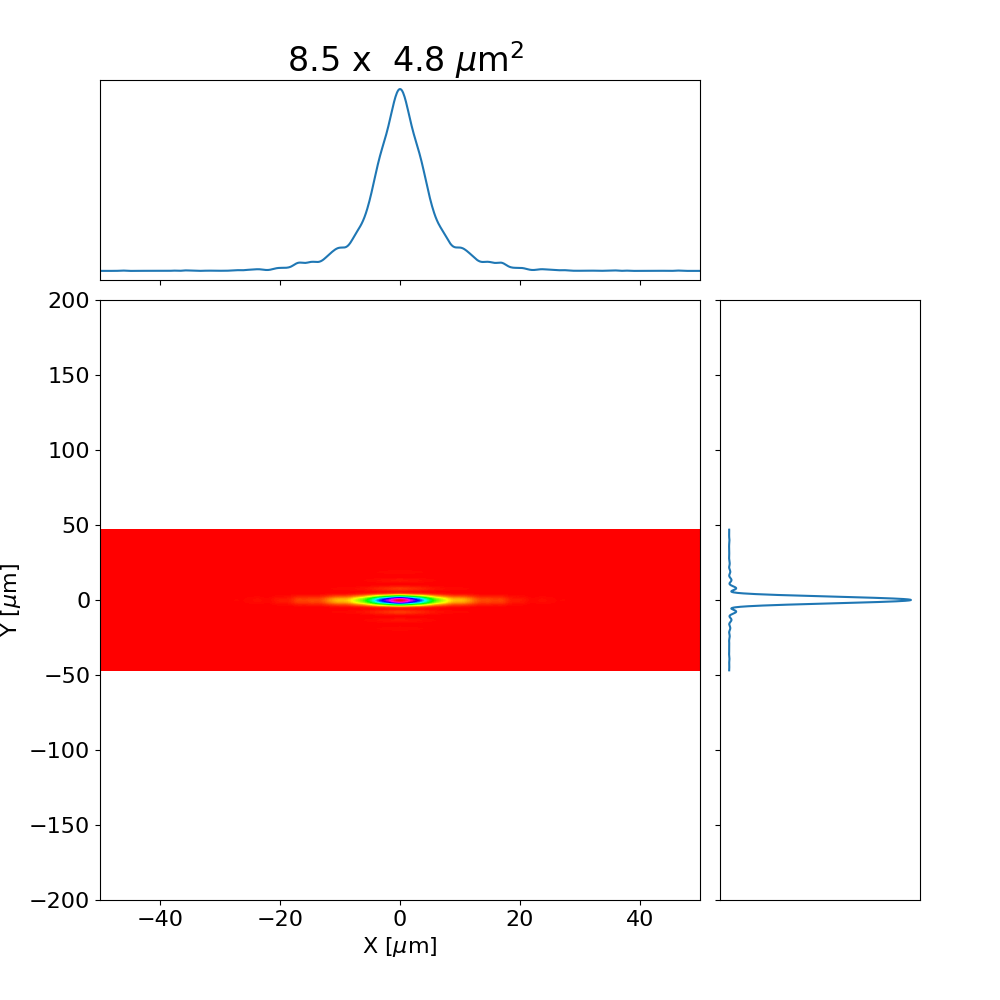
\includegraphics[width=0.45\textwidth]{figures/case1_wofry_ws_results.png}
    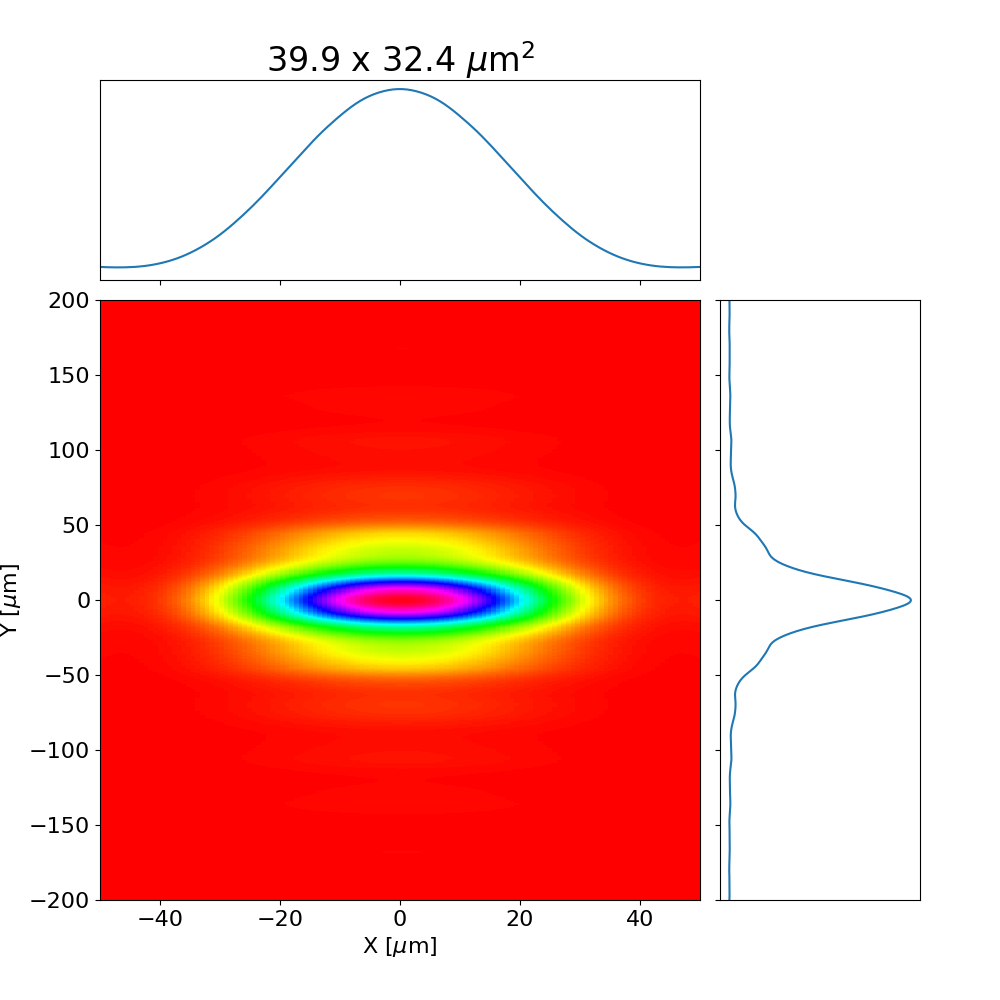
\includegraphics[width=0.45\textwidth]{figures/case2_wofry_ws_results.png}\\
    case 3~~~~~~~~~~~~~~~~~~~~~~~~~~~~~case 4\\
    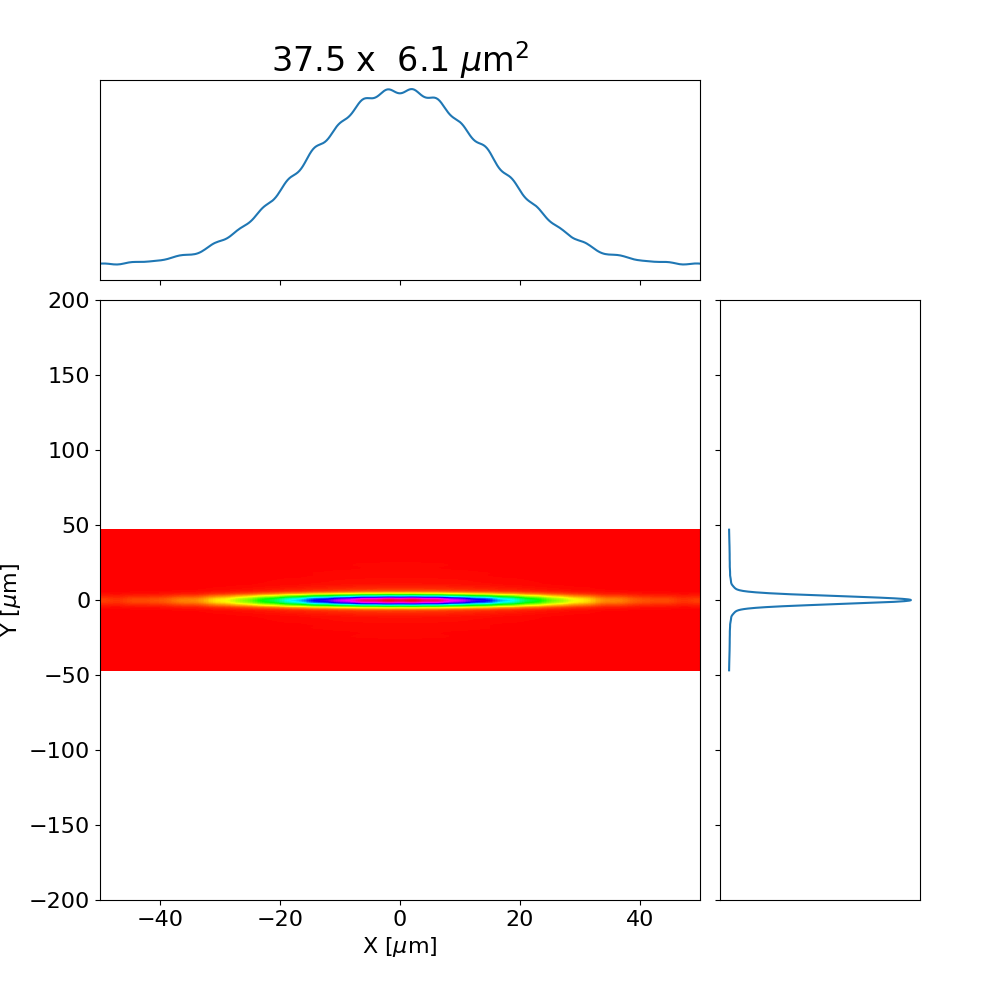
\includegraphics[width=0.45\textwidth]{figures/case3_wofry_ws_results.png}
    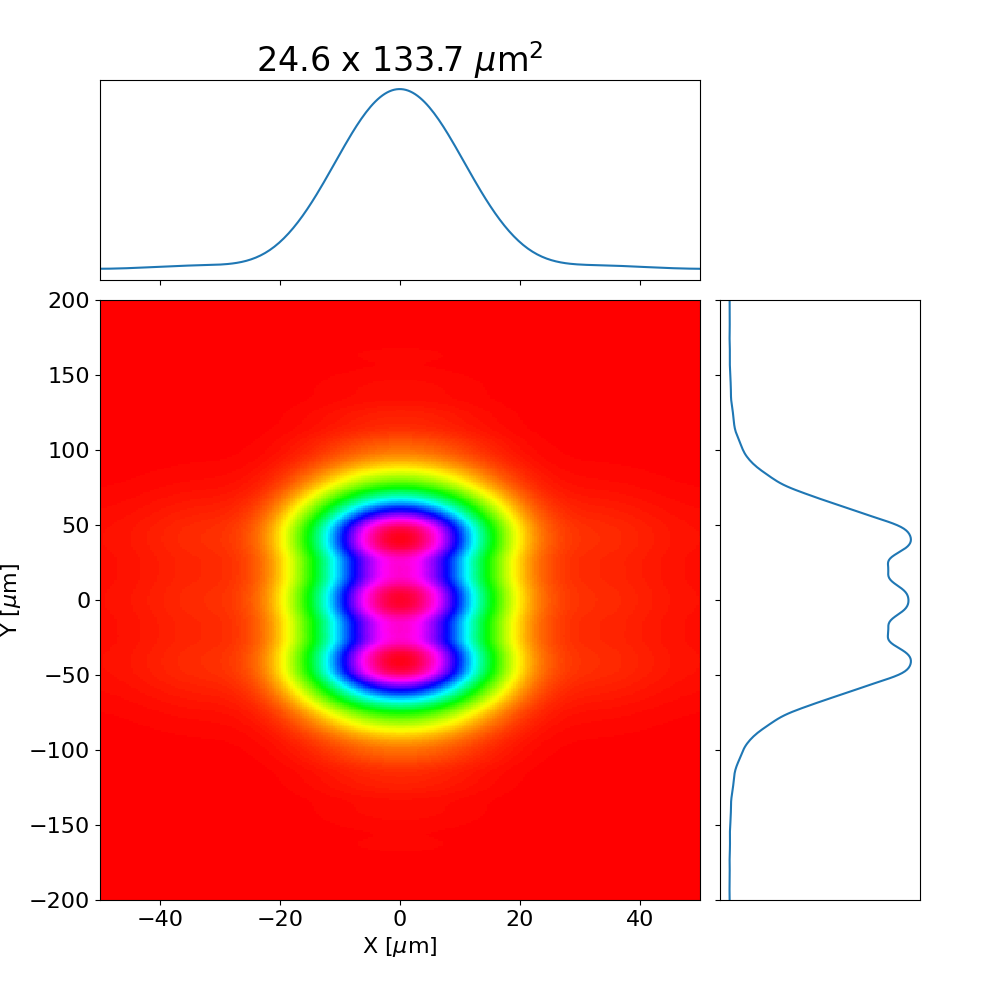
\includegraphics[width=0.45\textwidth]{figures/case4_wofry_ws_results.png}
    \caption{2D plots constructed from the 1D Wofry calculations.}
\end{figure}

\begin{figure}\label{fig:comsyl}
    \centering
    case 1~~~~~~~~~~~~~~~~~~~~~~~~~~~~~case 2\\
    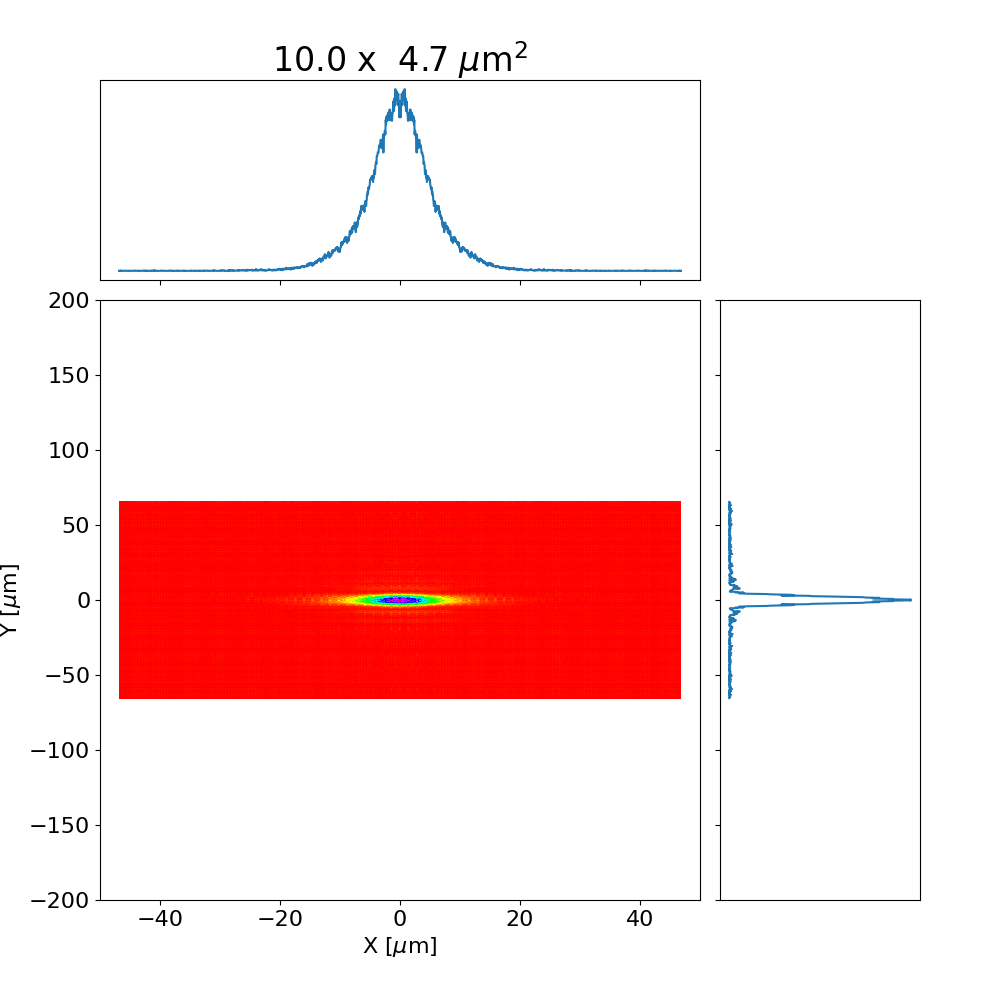
\includegraphics[width=0.45\textwidth]{figures/case1_comsyl.png}
    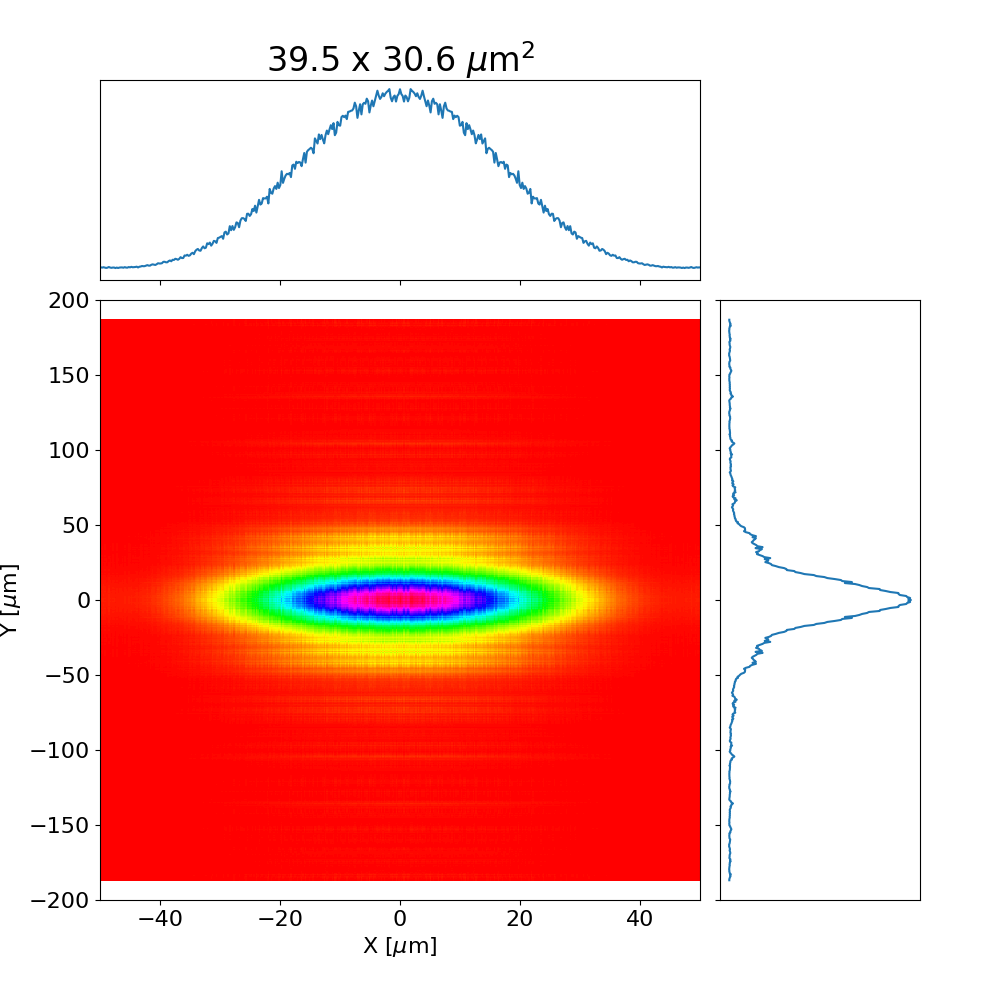
\includegraphics[width=0.45\textwidth]{figures/case2_comsyl.png}\\
    case 3~~~~~~~~~~~~~~~~~~~~~~~~~~~~~case 4\\
    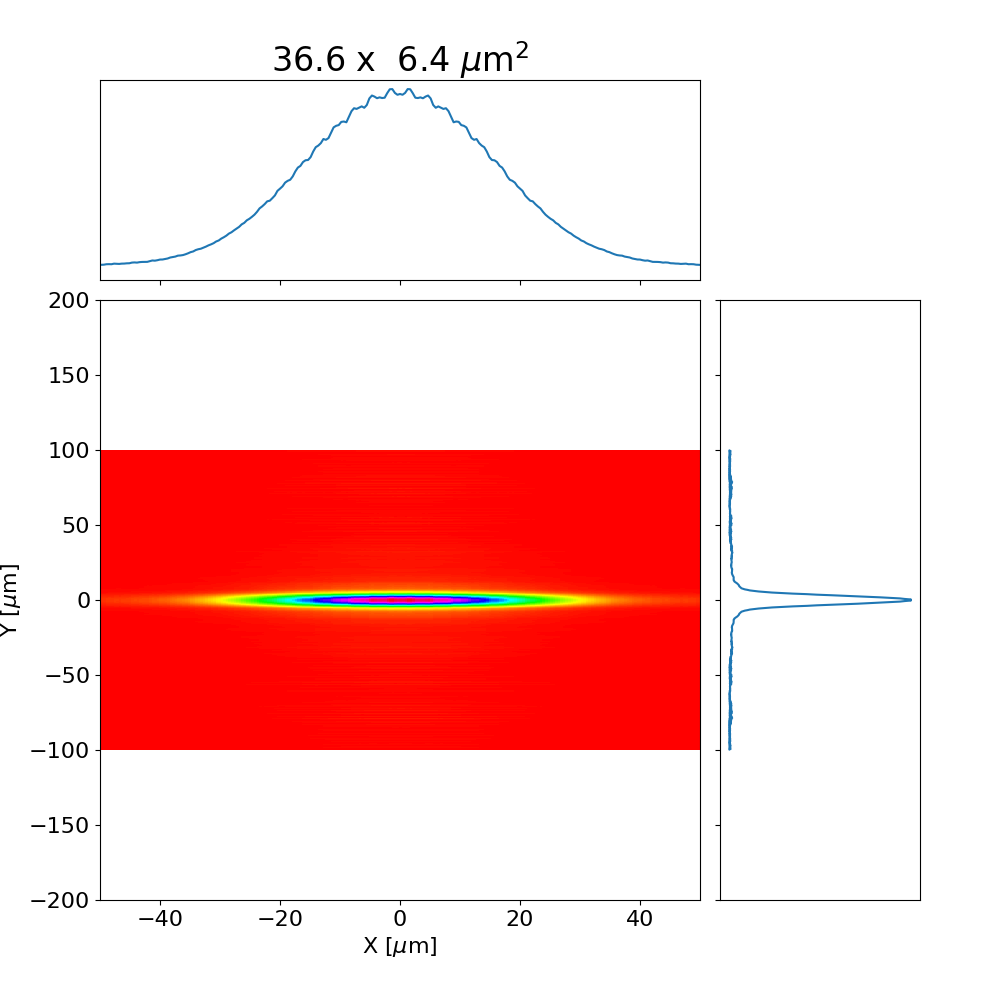
\includegraphics[width=0.45\textwidth]{figures/case3_comsyl.png}
    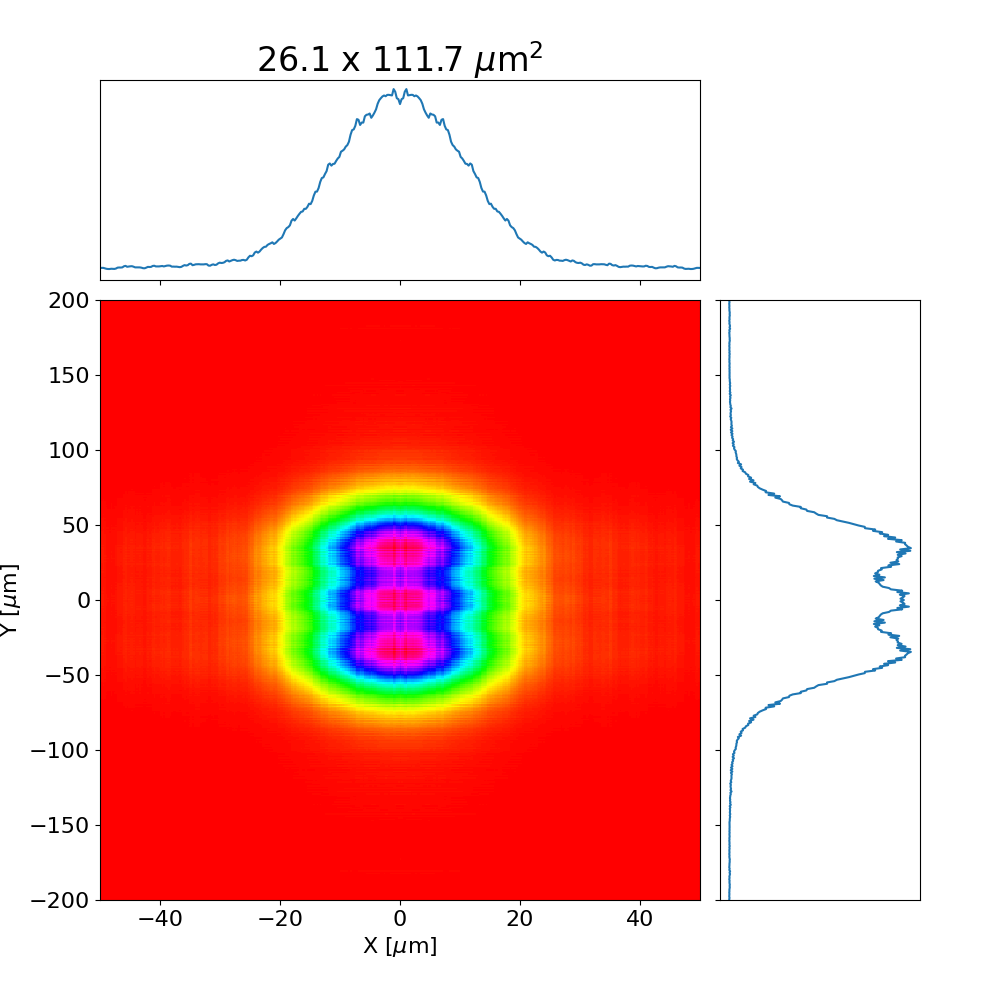
\includegraphics[width=0.45\textwidth]{figures/case4_comsyl.png}
    \caption{COMSYL calculations}
\end{figure}

\begin{figure}\label{fig:srw}
    \centering
    case 1~~~~~~~~~~~~~~~~~~~~~~~~~~~~~case 2\\
    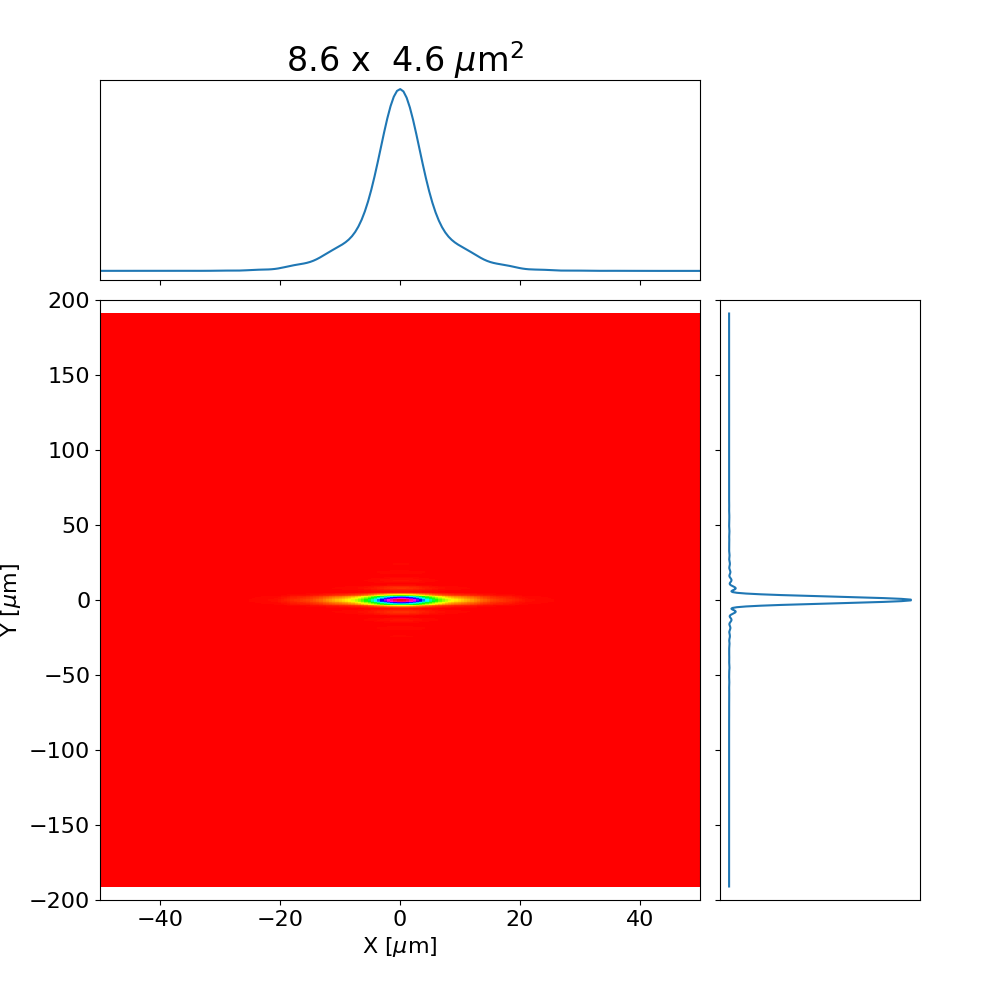
\includegraphics[width=0.45\textwidth]{figures/case1_srw.png}
    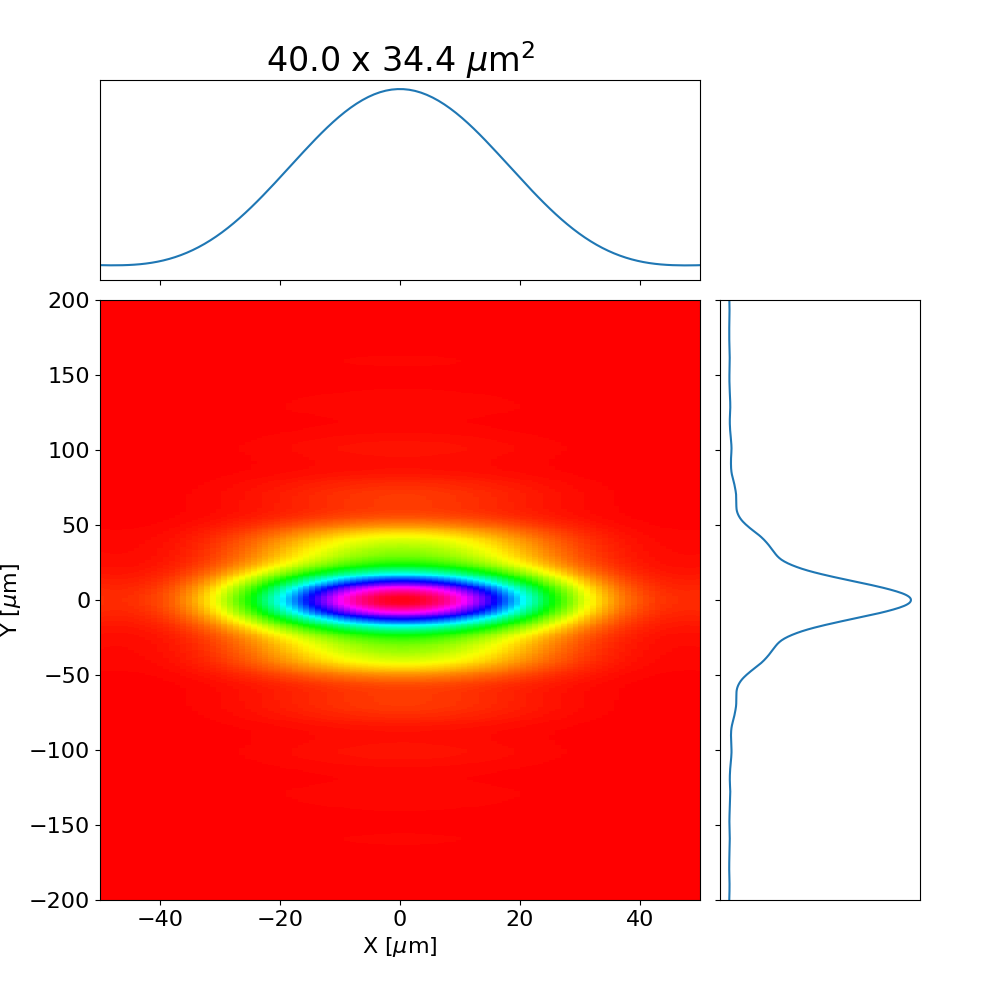
\includegraphics[width=0.45\textwidth]{figures/case2_srw.png}\\
    case 3~~~~~~~~~~~~~~~~~~~~~~~~~~~~~case 4\\
    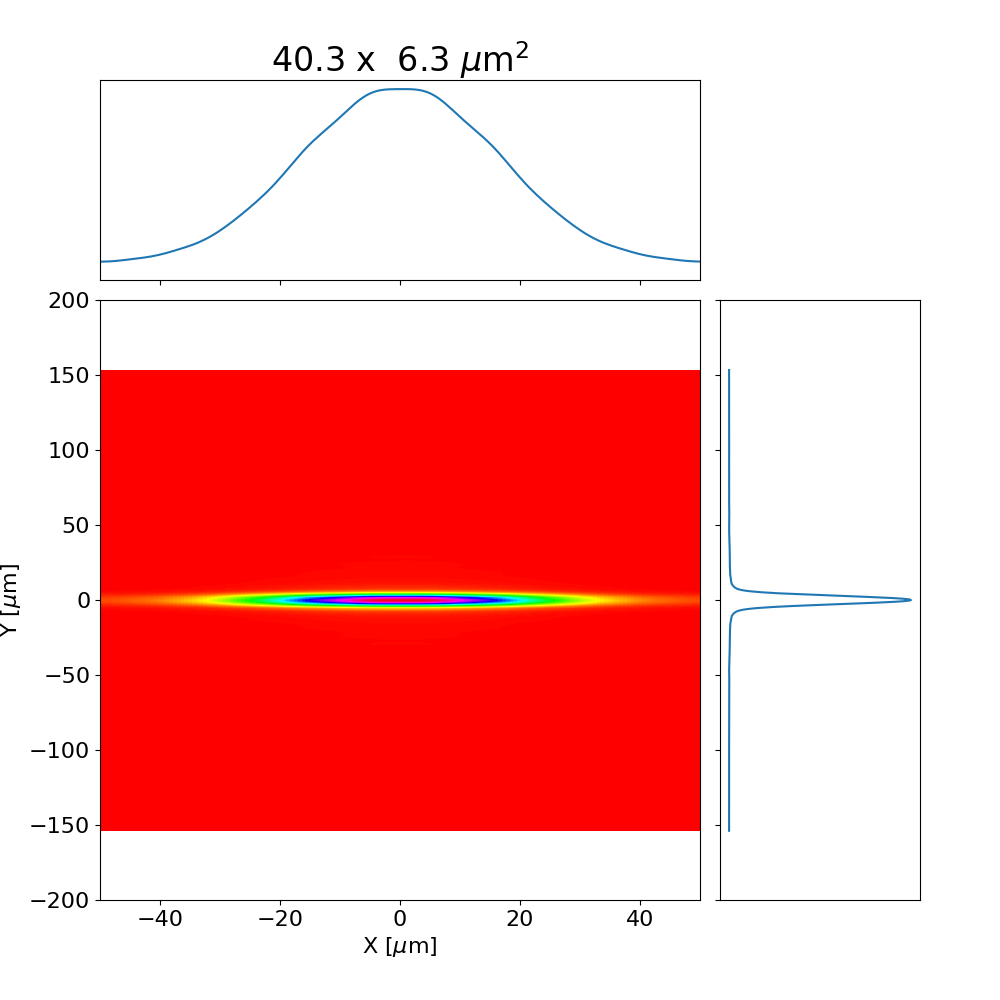
\includegraphics[width=0.45\textwidth]{figures/case3_srw.png}
    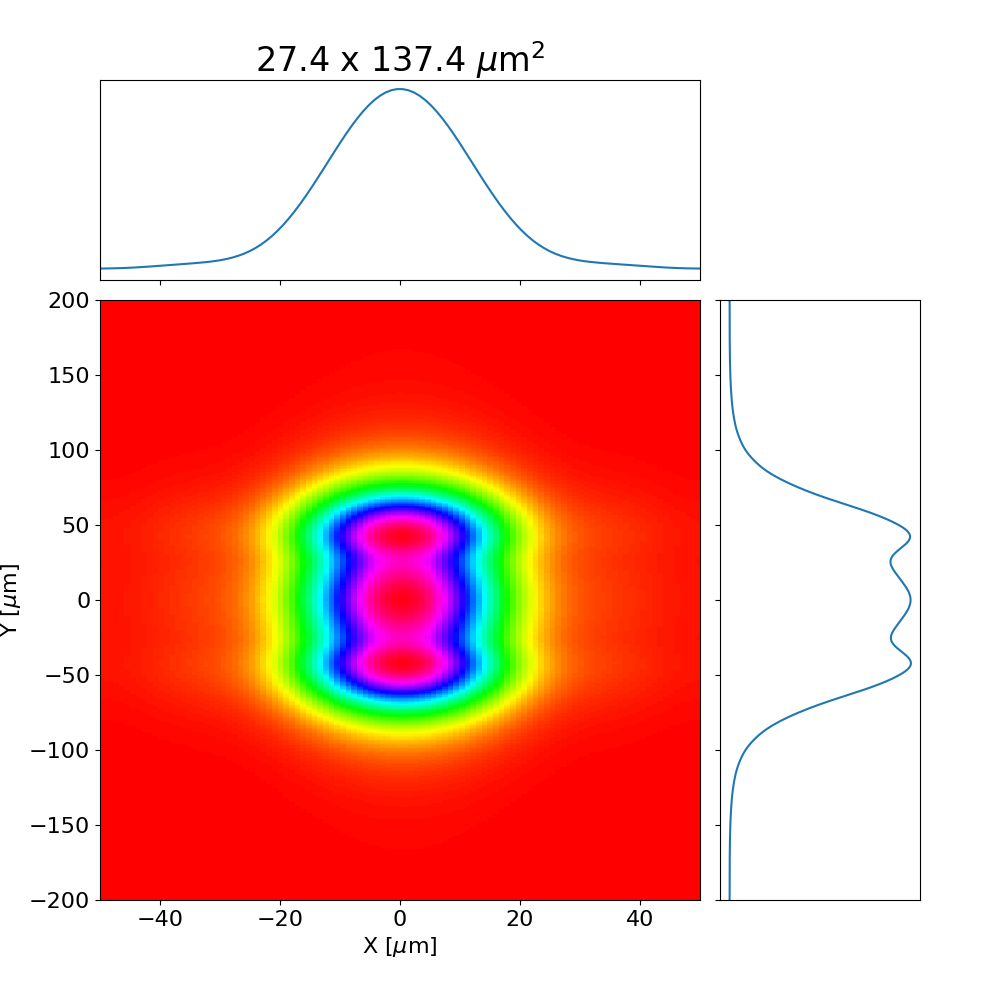
\includegraphics[width=0.45\textwidth]{figures/case4_srw.png}
    \caption{Multi-electron SRW simulations}
\end{figure}

\vspace{3cm}

\begin{figure}
    \label{fig:hybrid}
    \centering
    case 1~~~~~~~~~~~~~~~~~~~~~~~~~~~~~case 2\\
    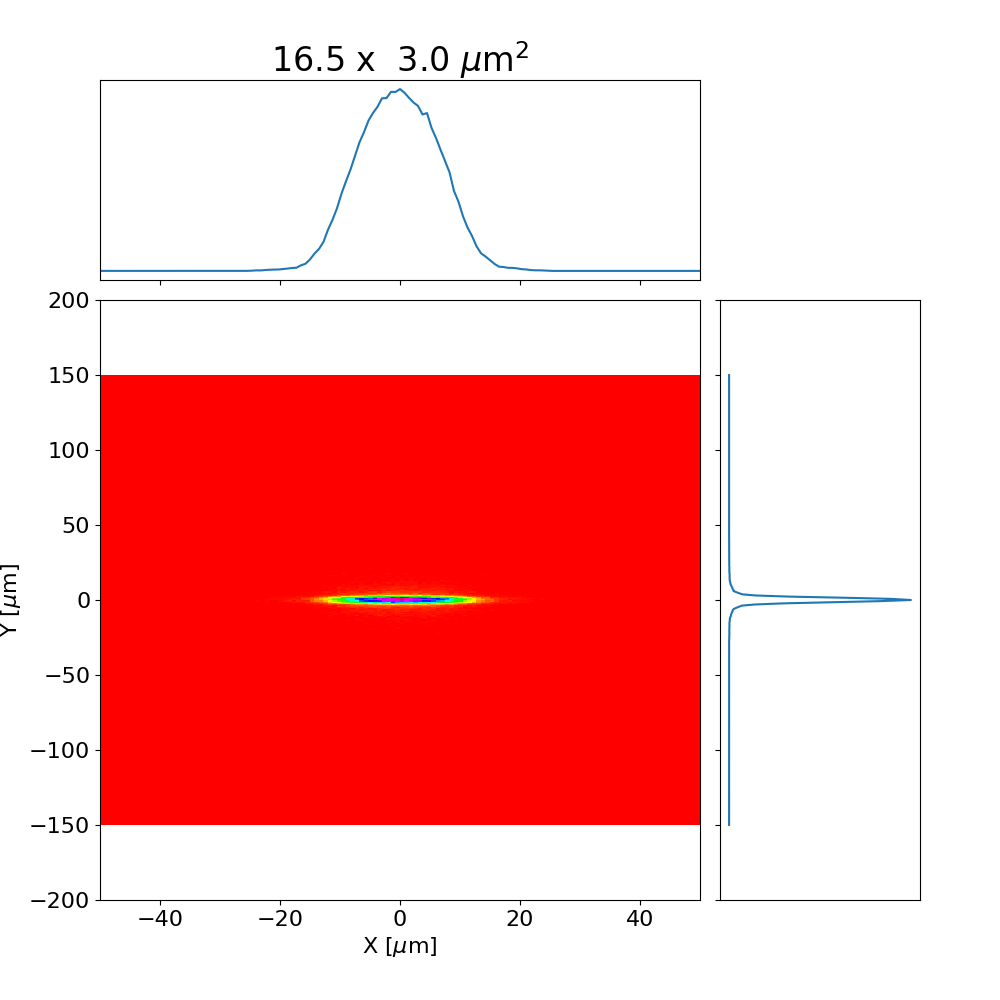
\includegraphics[width=0.45\textwidth]{figures/case1_hybrid.png}
    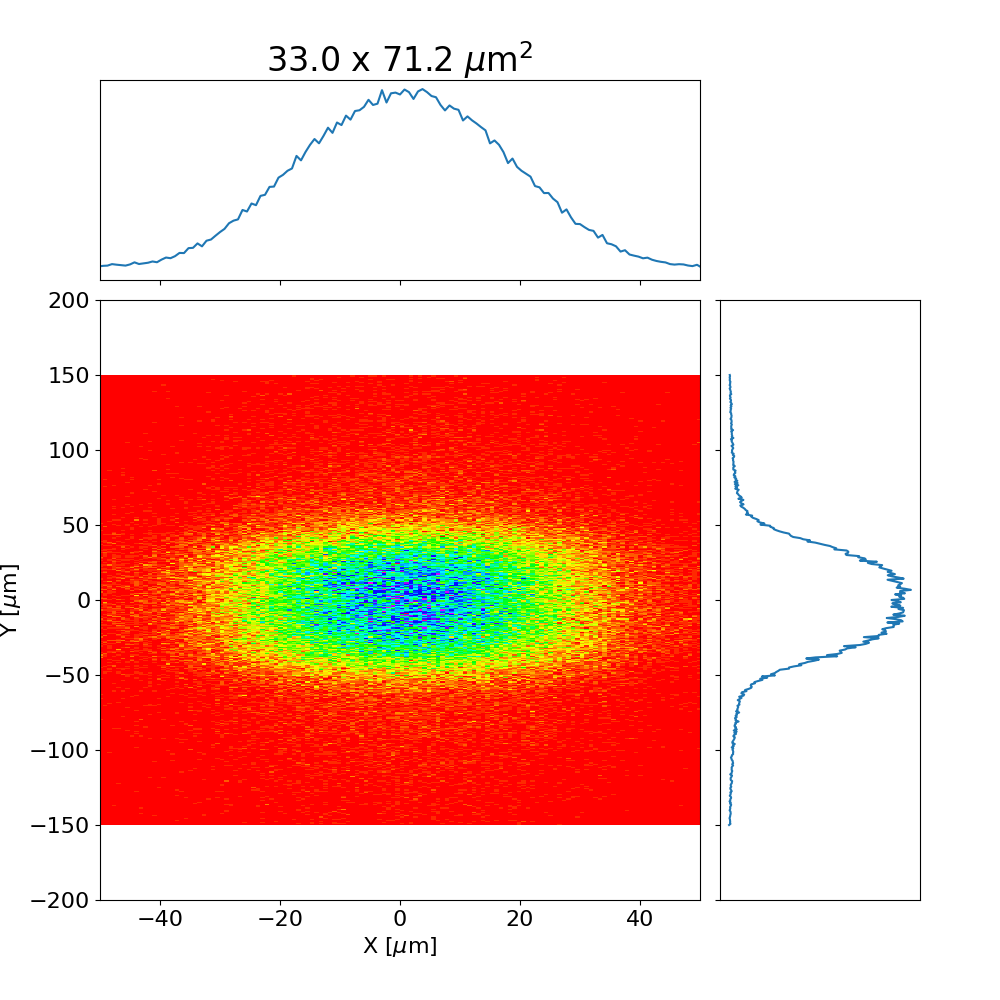
\includegraphics[width=0.45\textwidth]{figures/case2_hybrid.png}\\
    case 3~~~~~~~~~~~~~~~~~~~~~~~~~~~~~case 4\\
    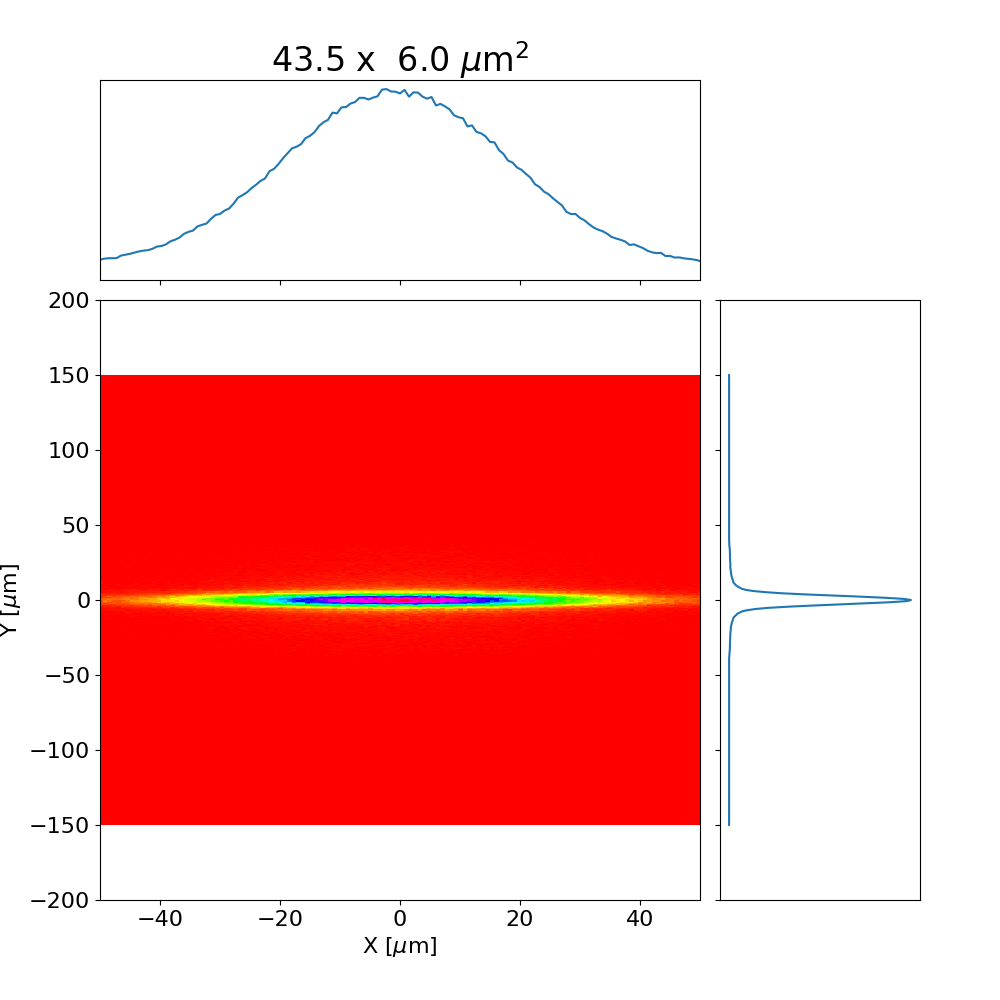
\includegraphics[width=0.45\textwidth]{figures/case3_hybrid.png}
    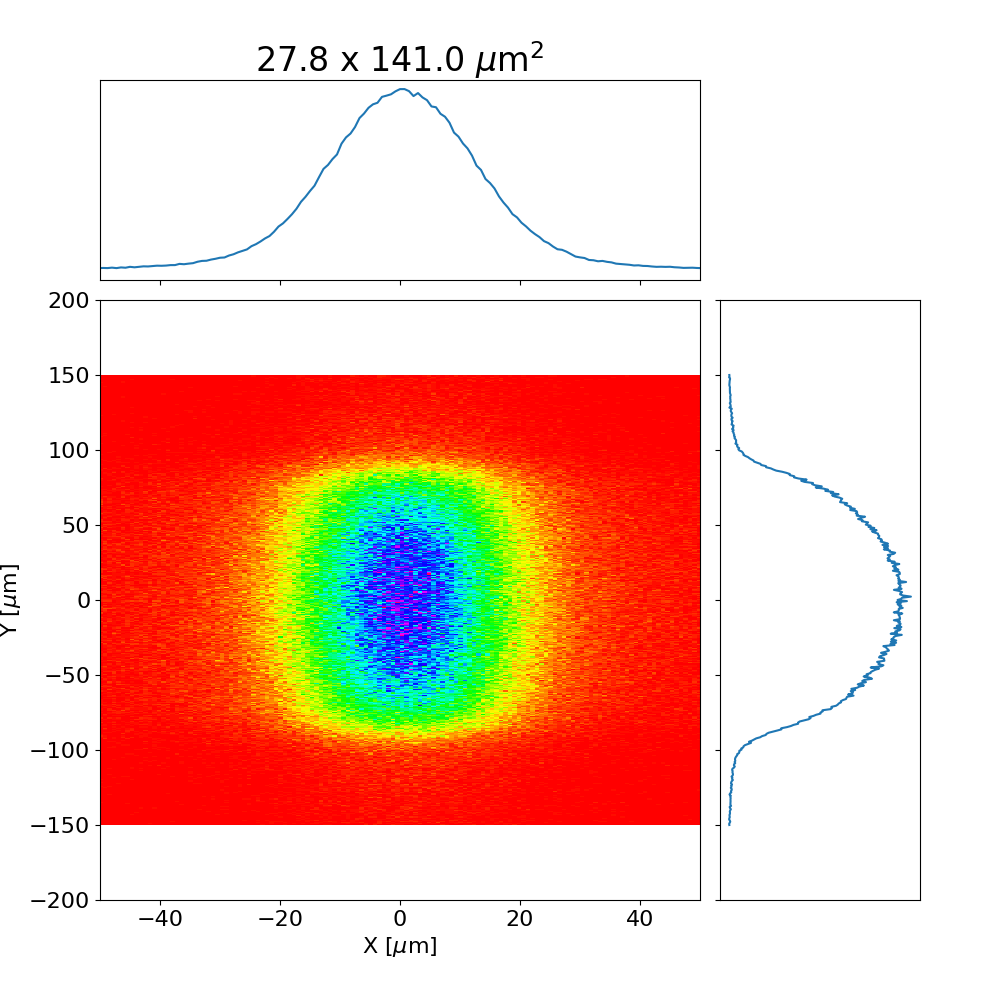
\includegraphics[width=0.45\textwidth]{figures/case4_hybrid.png}
    \caption{Hybrid ray tracing simulations}
\end{figure}

\newpage


\section{Discussion}
\label{sec:discussion}

\subsection{f1 f2 trajectories and focal sizes} 

From the results shown in the last section, it is clear that the focusing of the partial coherence x-ray beams produced by low emittance storage rings, is a complex phenomenon as the effects of diffraction induced by coherence modify the propagation of the beam. The concepts of geometrical optics often used to calculate the focal position (lens equation) and the focal size (using magnification) fail when the x-ray beam is cropped significantly (NA reduced) (see Figs.~XX, XX) . In older synchrotrons, these analytical results from geometrical optics work better because the beam is mostly incoherent in the horizontal, therefore a pinhole source is then created usually after imaging the source into a secondary source at the pinhole position. The systems studied here will image directly the source into the focal plane, using two focusing elements (paired transfocators) and this is an innovative concept permitted only in new storage rings. However, at the ID18 beamline at the EBS-ESRF source, and at the energy discussed of 7 keV, the horizontal coherent fraction is still much lower than the vertical one (Fig. XX). This imply the necessity of cropping more the beam in horizontal than in vertical to get the same CF, therefore its smaller reduction of NA induces more distortions in the beam. In the vertical direction, the beam must be cropped as well, and the beam distortion is smaller than in horizontal. However, the apertures needed to obtain typical values of CF suitable for experiments (50-95 \%) do strongly affect the evolution of the beam, but still they are large enough to justify to consider a secondary source at the slit. 
This is evident in Fig. 3: in vertical most of the typical apertures (up to XX um) still makes the system to image the source at the ID center to the focal plane, whereas in horizontal, the cropping needed to get $CF_h=$ 90\% already makes the effect of "shifting" the source from its real position (ID center) to the slit position. Although this shift of the focal position has been predicted and calculated before (see \cite{tanaka} for Gaussian beams, or \cite{whej} for synchrotron beams) our calculations in Fig. 3 reveal two important facts: i) the shift exists but it is directed upstream to the position defined by the geometrical optics for the slit image (and not downstream to the lens position, as found for the systems analyzed in the references mentioned), and ii) the focal size is highly degraded (its size increases) when the beam focus is found in between the two positions defined by the geometrical optics.  


Pairing two transfocators consists in matching their focal distances to guarantee the focus at the desired focal plane (the sample position). By matching the lens equations of the two lenses, it is possible the analytical expression in Eq. XX permits to calculate f2 as a function of f1. This can be done for the two cases: with the source at the ID center (limit of high NA, no cropping) of with the source at the slit (pinhole limit when NA$\arrow$0). The analytical equations diverge at the point where lens 1 focuses onto f2.
\inblue{Looking at Fig.~\ref{fig:f1f2map}a we observe an asymptotic approach (for $f1<$~\SI{25}{\meter} or $f1>$~\SI{70}{\meter}) of the numerical results to geometrical optics results, mostly with source at the ID, but sometimes (with closed slit) to the case of the source at the slit position. However, this case is obtained in H with a reasonable aperture $a=$~\SI{40.4}{\micro\meter}, a value of interest in real cases (to get $CF_h=$90\%) but with a less interesting aperture in V $a=$~\SI{25}{\micro\meter}, because high coherence can be obtained with more opened slits without compromising transmission. }
Our numerical simulation of the (f1,f2) trajectory maps present two characteristics: i) they asymptotically match the analytical positions for sufficiently high of small $f_1$, either the position obtained when the source is at ID (high NA ) or when the source is at the slit (low NA), and ii) the analytical singularities found in $f_2$ when lens 1 focuses on lens 2 is smoothed and the transition from one branch to another becomes soft. It is softer for smaller NAs in the horizontal (Fig. 4a) but not relevant in the vertical (Fig. 4b). The inflexion point shifts from the position "ID center" to the "slit center" when NA reduces. But, as discussed in the last paragraph, this shifting is evident in the horizontal for the usual slit openings, but is not yet relevant in vertical for common apertures. 

When looking at the obtained sizes in Fig.~\ref{fig:focalSizes} the results of the geometrical optics cannot be used to guess the spot sizes. In H, only around $f_1\approx$~\SI{30}{\meter} geometrical optics give good results. In V, at  $f_1 <$~\SI{30}{\meter} the geometrical optics prediction can be reliable. 
 

% The trajectory maps and size graphs are complex. First beamline that gets high coherence by direct imaging the source in H at 4th generation storage ring sources. 



    
\subsection{Methods of caculation}

The results presented here in Fig. 5 contains hundreds \todo{how many} of individual simulations. Each point or simulation implements a full partial coherence simulation involving the transport of many modes. This has only be possible with the development of a new fast 1D CMD method that has been outlined in section XX. Section XX makes a careful analysis of several points in Fig. XX and XX, and also validates the accuracy of the Wofry 1D method by comparing the results with full 2D CMD and SRW-ME. 
The wave optics simulations using the three methods (Wofry1D, COMSYL and SRW) give the same results within a \todo{10\%??} discrepancies. This is a validation than the newly proposed method Wofry1D produces reliable results in a much shorter calculation time \todo{table/discussion on CPU usage?}. Note that these numerical values depend not only on the method used, but also on the particular specific parameters in each method (number of pixels for sampling, zoom factor in propagation, etc.). However, the agreement is very good in terms not only of numerical values but also in the shape of intensity distributions (compare Figs. XX).
 
\inred{In our search of fast and accurate methods of calculation, based on out scheme of making hierarchical simulations \cite{hierarchical} we have applied the hybrid. We see that the results are acceptable in terms of calculated beam sizes, ... }

\todo{run times comparison. Table?}

\subsection{Further simulations}

\begin{itemize}
    \item{\todo{compare flux values with all methods: }}
    
    \item \todo{briefly discuss correction to the thermal load by M1 and DCM. Check correction of the fitted curvature and degradation by the residual errors}
    
    \item discuss the real combination of lenses that will be used to match the R in the simulations. Justify the approximation of using a single lens with a given R. 
    
    \item Out of resonance discussion
    
\end{itemize}


\begin{table}[]
    \label{table:absorption}
    \caption{Comparison of beam intensity attenuation in percent by the slit, lens 1 and lens2.
    \todo{SRW calculations are single electron, using diameter 1mm and thickness 30 um TO UPGRADE...}
    \todo{remove this table?}
    }
    \centering
    \begin{tabular}{c|c|c|c|c}
case  & Wofry1D & COMSYL  & SRW& Hybrid \\
1     & 0       & 0       & 96.7,4.4,16.7   & 0 \\
2     & 0       & 0       & 96.7,3.5,2.4   & 0 \\
3     & 0       & 0       & 85.4,3.6,10.1   & 0 \\
4     & 0       & 0       & 85.4,5.4,2.6    & 0 
    \end{tabular}
\end{table}


\subsection{Tips to experimentalists}

\begin{itemize}
    \item \todo{because of the system complexity it would be good to have an experimental method to guarantee that the focus sit on the image plane (so we are not out of focus)}
    \item Useful plots: CF vs slit size, trajectories, size. Simulated ones, create similar look-up tables. Digital twin. 
    \item To get similar size, prefer a large $f_1$ to avoid too large illumination in lens2.
    \item Lens granularity
\end{itemize}



\section{Summary and conclusions}
\label{sec:summary}

We have studied in detail the focusing of a partial coherent beam (as produced by the low emittance storage ring EBS-ESRF) by a system of one and two transfocators (or lenses). In agreement with existing works, we observe a displacement of a focal position originated by the reduction of NA. The reduction of NA is the result of closing a slit to gain coherence, a usual procedure in beamlines for X-ray coherence applications. We observed that good focusing (small focus) is obtained when its position coincide with the positions predicted by the geometrical optics (considering the source either at the ID position or at the slit position) but not in intermediate positions (Fig.~\ref{fig:oneTFundPartialCoherence}??)/

We calculated numerically the map or trajectory of focal distances $(f_1,f_2)$ needed to maintain the focus at the image plane. The beam size values obtained for different cases are very different of the ones predicted by the geometrical optics.  

Numerical calculations for this work have been done using a newly developed method of coherent mode decomposition in 1D. This method is very fast, and many simulations can be run in a laptop, therefore it is idoneous for parametric calculations as presented here. This method is available in the Wofry add-on of the OASYS\cite{codeOASYS} suite. Four cases are also calculated and compared among them using the other methods available in OASYS, like the full 2D coherent mode decomposition using COMSYL \cite{codeCOMSYL}, the OASYS interface for the SRW \cite{codeSRW} code, and ray tracing with SHADOW\cite{codeSHADOW} using the hybrid method proposed by \cite{codeHYBRID}. OASYS workspaces for the simulations performed in this paper are available at {\tt https://github.com/oasys-esrf-kit/...} 


% Pairing two transfocators permits to create a focal spot with size that can adapt to the sample dimensions. The transfocators are design to focus the beam to a spot of variable size in a given interval for a large photon energy range. 

% For this analysis, we have developed an innovative algorithm for fully describing partial coherence from undulator beams using coherent mode decomposition.

% This method is based on the separated analysis of the horizontal and vertical directions (1D model). The results are compared with fully 2D methods (SHADOW hybrid \cite{XX}, SRW \cite{XX}, COMSYL \cite{XX}). We apply the results to the study of a two transfocator system that is being designed for the new ID18 beamline at the upgraded EBS-ESRF \cite{XX}.  

\newpage

%%%%%%%%%%%%%%%%%%%%%%%%%%%%%%%%%%%%%%%%%%%%%%%%
%%%%%%%%%%%%%%%%%%%%%%%%%%%%%%%%%%%%%%%%%%%%%%%%
%%%%%%%%%%%%%%%%%%%%%%%%%%%%%%%%%%%%%%%%%%%%%%%%
\appendix

%%%%%%%%%%%%%%%%%%%%%%%%%%%%%%%%%%%%%%%%%%%%%%%%


%%%%%%%%%%%%%%%%%%%%%%%%%%%%%%%%%%%%%%%%%%%%%%%%
\section{One lens: comparison of methods}
\label{appendix:comparison}


% \begin{figure}
%     \centering
%     \includegraphics[width=0.95\textwidth]{figures/oneTFund_400um.eps}
%     % \includegraphics[width=0.95\textwidth]{figures/oneTFund_300um.png}  
%     \includegraphics[width=0.95\textwidth]{figures/oneTFund_200um.eps}
%     % \includegraphics[width=0.95\textwidth]{figures/oneTFund_100um.png}

%     \caption{Evolution of the size of a coherent undulator beam cropped by a slit and focused by a lens of different radii values $R$: a) \SI{400}{\micro\meter} and b) \SI{200}{\micro\meter}.
    
%     }
%     \label{fig:oneTFundAppendixR}
% \end{figure}


\begin{figure}
    \centering
    
    a) Und + RectSlit + RealLens \\
    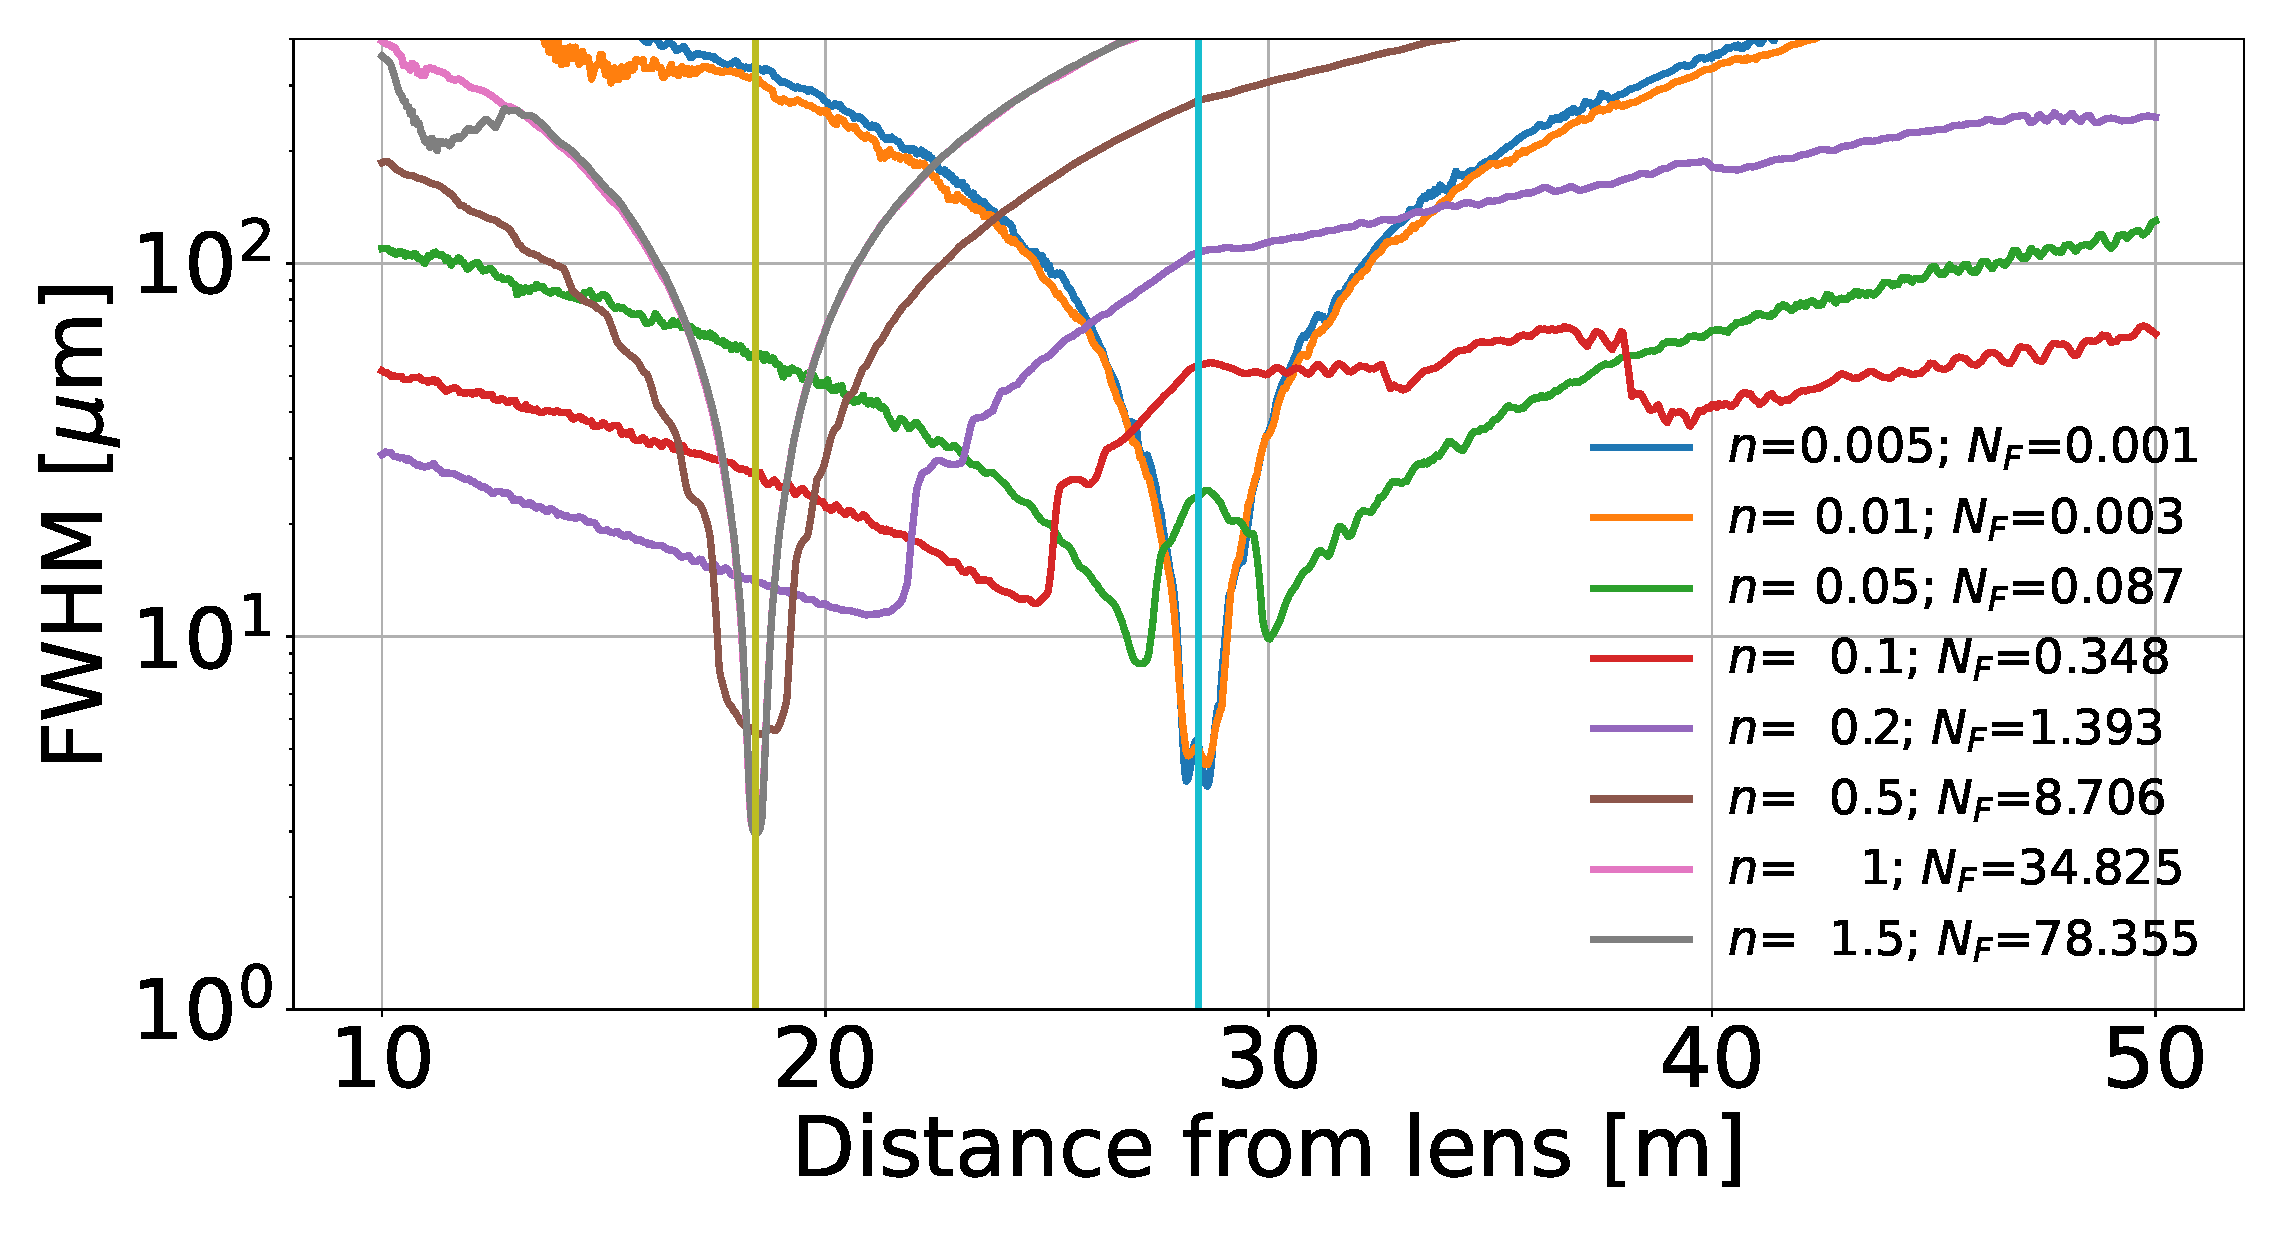
\includegraphics[width=0.95\textwidth]{figures/oneTF_UndSource_RectSlit_R200um.eps}
    
    b) Gauss + RectSlit + RealLens \\
    \includegraphics[width=0.95\textwidth]{figures/oneTF_GaussianSource_RectSlit_R200um.eps}
    
    c) Gauss + GaussSlit + RealLens \\
    \includegraphics[width=0.95\textwidth]{figures/oneTF_GaussianSource_GaussianSlit_200um.eps}

    d) Gauss + GaussSlit + IdealLens \\
    \includegraphics[width=0.95\textwidth]{figures/oneTF_GaussianSource_GaussianSlit_IdealLens.eps}
    
    e) Hybrid (Und + RectSlit + RealLens) \\
    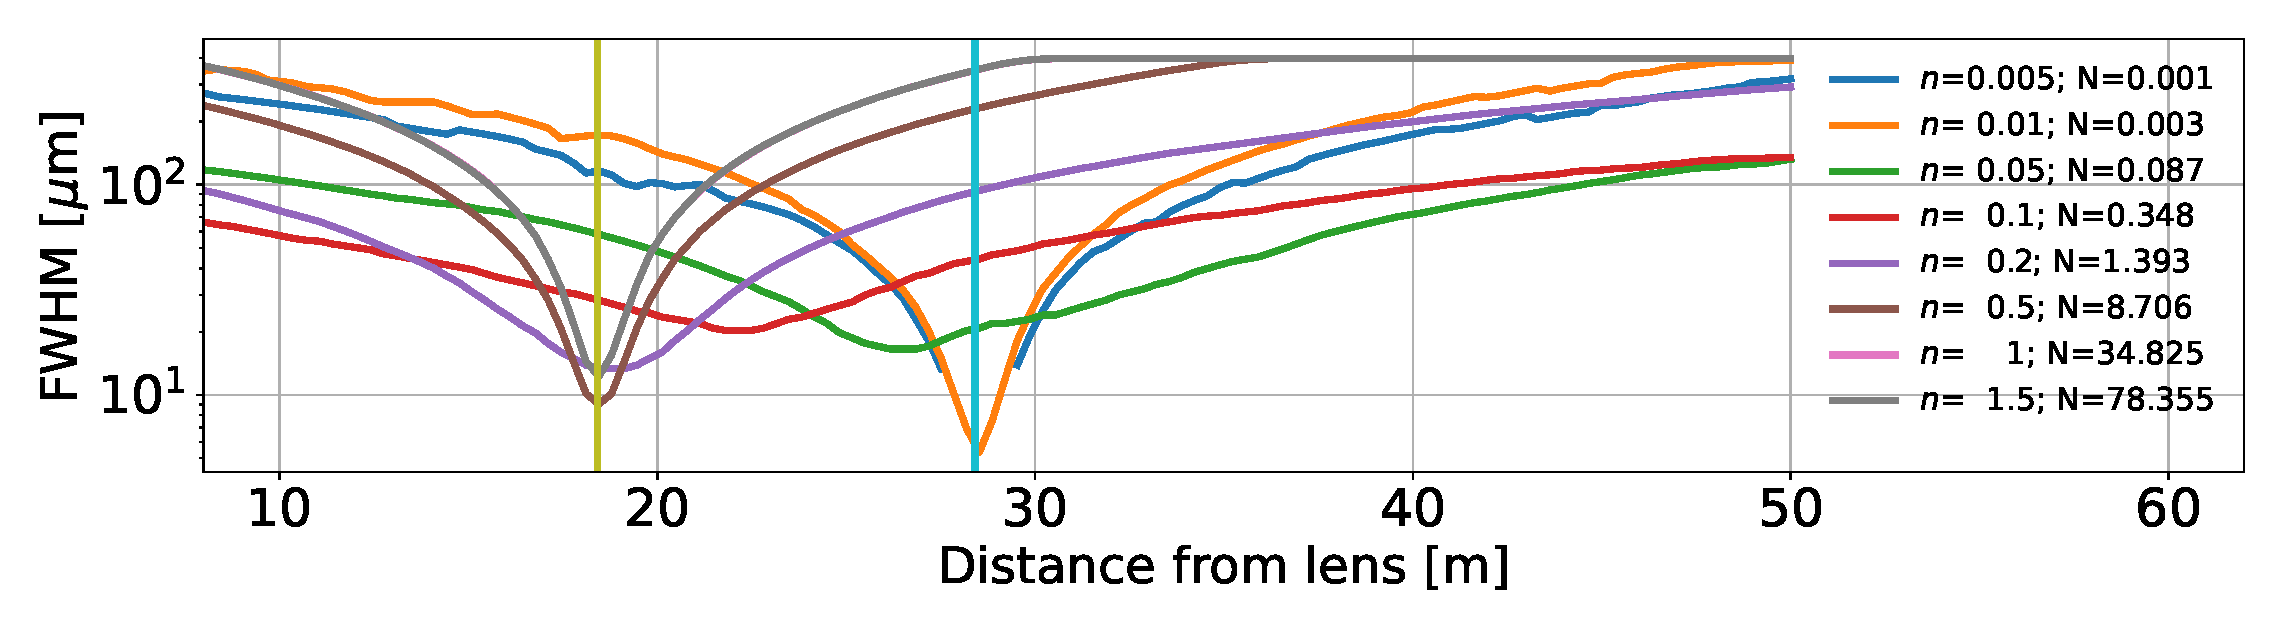
\includegraphics[width=0.95\textwidth]{figures/oneTF_ShadowHybrid_R200um.eps}
    
    \caption{Evolution of the size of a coherent undulator beam cropped by a slit and focused by a lens of $R$=~\SI{0.2}{\milli\meter} using different methods: 
    
    a) Undulator source + Rectangular Slit + Real Lenses
    
    b) Gaussian source + Rectangular Slit + Real Lenses
    
    c) Gaussian source + Gaussian Slit + Real Lenses
        
    d) Gaussian source + Gaussian Slit + Ideal lens (Full Gaussian)
        
    e) Ray tracing, hybrid, with undulator source + Rectangular Slit + Real Lenses.
    }
    \label{fig:oneTF_comparison}
\end{figure}


\begin{figure}

    \includegraphics[width=0.95\textwidth]{figures/waist_size_comparison.eps}
    
    \caption{Waist size vs slit aperture for the different methods studied. 
    
    }
\end{figure}

\section{SRW results for pairing two lenses}
\label{appendix:srw}
xxxx

\section{Hybrid results for pairing two lenses}
\label{appendix:hybrid}

\begin{figure}
    \centering

    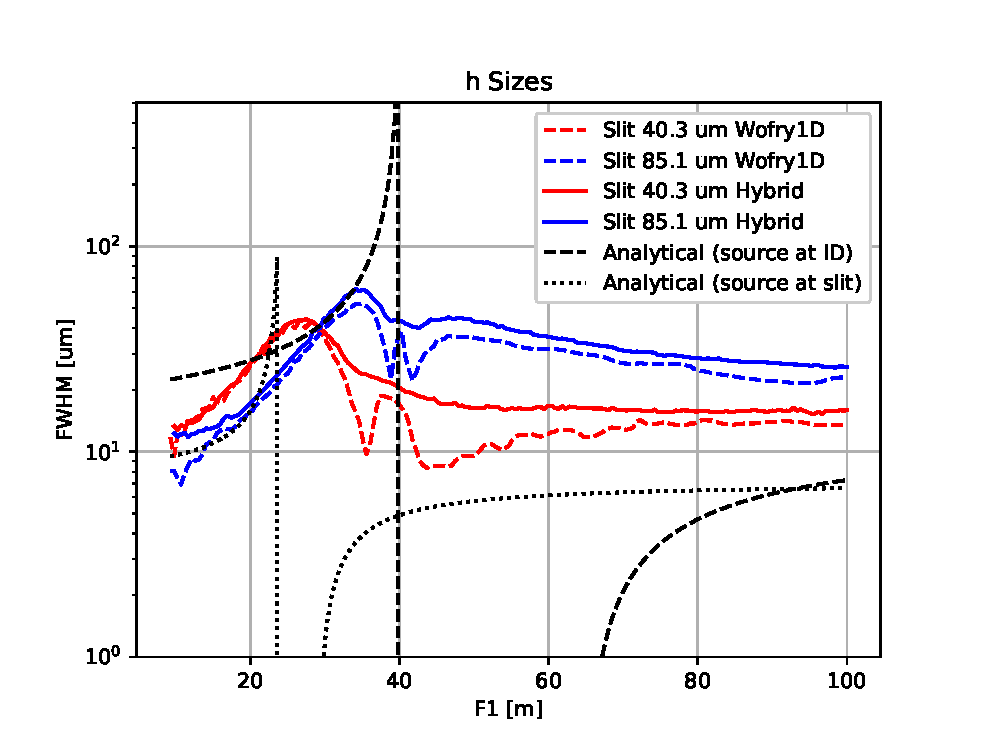
\includegraphics[width=0.95\textwidth]{figures/sizes_h_hybrid.eps}
    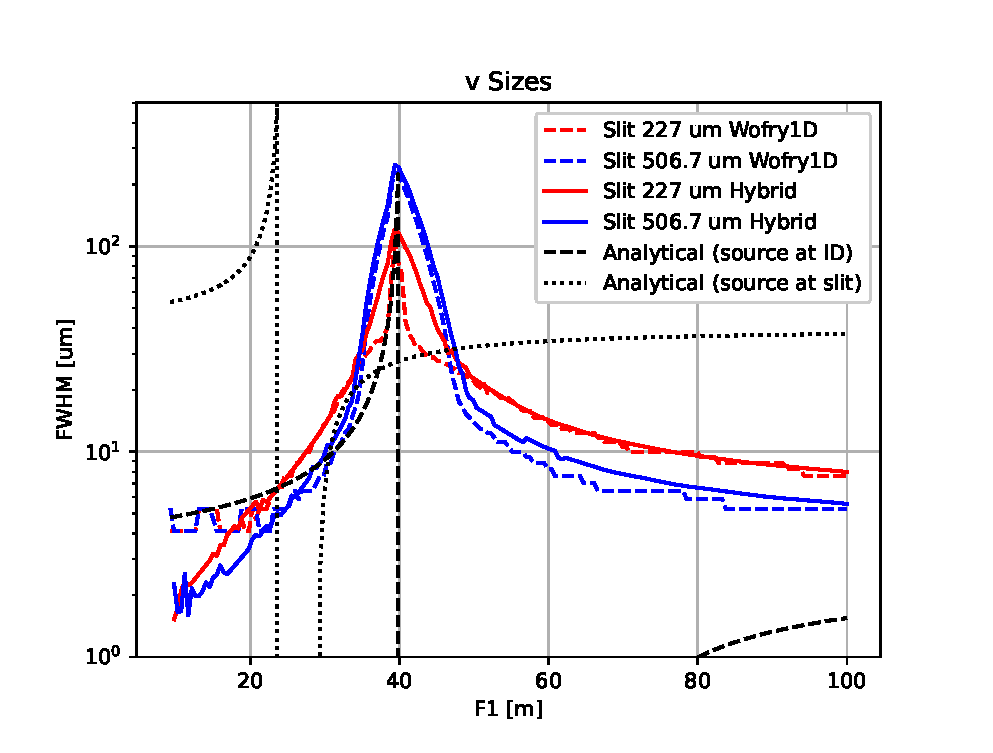
\includegraphics[width=0.95\textwidth]{figures/sizes_v_hybrid.eps}
        
    \caption{Focal sizes obtained by hybrid ray tracing method, for two slit aperture cases, compared with 1D Model (WOFRY). Analytical values are same as Figure \ref{fig:focalSizes}. 
    }
    \label{fig:focalSizes_hybrid}
\end{figure}

% %%%%%%%%%%%%%%%%%%%%%%%%%%%%%%%%%%%%%%%%%%%%%%%%
% \section{OLD PART FOR ONE LENS}

% We have calculated the beam evolution using wave optics. The source has $\sigma_s=$\SI{15.3/2.355}{\micro\meter} and $\lambda=$\SI{1.2}{\AA}, and the lens $p=$\SI{65}{\meter}, $f=$\SI{28.2}{\meter}, and a slit of variable aperture $a$ is placed at $p_a$=\SI{30}{\meter} from the lens. The beam at the slit plane has a size $\sigma_a=$\SI{125}{\micro\meter} \todo{CHECK WITH FORMULAS...} and the aperture is open at $a = n \sigma_a$ with $n=6,4,2,1.5,1,0.5,0.2,0.1$. The cross section of the beam is defined by i) the full-width at half-maximum (FWHM) of the intensity distribution, or also ii) the on-axis intensity $I_{axis}$. At the focal position, the FWHM should present a minimum and $I_{axis}$ a maximum. 

% The slit is implemented in two ways. First, as a Gaussian appodization window for the beam intensity. This guarantees the validity of regime (2) in the previous section. The FWHM of the weighting  Gaussian window corresponds to the slit aperture $a$. This is the value that better approximates a slit by a Gaussian window, as discussed in Appendix~\ref{sec:appendixC}. Second, in a  more realistic model, the slit is acting as a transmission window of rectangular shape with width $a$. 

% Fig.~\ref{fig:oneTFG}a shows the evolution of the beam after being focused by the lens. With the open slit the geometrical optics give a focal position $q=$\SI{49.81}{\meter} (source at $p$) and $q'=$\SI{470}{\meter} (source at $p_a$ slit). \todo{CALCULATE AND COMPARE FOCAL SIZES} 


% \begin{figure}
%     \centering
%     %\includegraphics[width=0.95\textwidth]{figures/FigureG_1.png}
%     \includegraphics[width=0.95\textwidth,height=5cm]{figures/FigureG_2.png}
%     \includegraphics[width=0.95\textwidth,,height=5cm]{figures/Figure_2.png}
%     \caption{Evolution of a beam cropped by a slit and refracted by a lens as a function of the distance from the lens.
%     %a) evolution of the FWHM of the beam size, 
%     The plot shows the evolution of the intensity on-axis. The aperture is open at $a = n \sigma_a$ with $n=6,4,2,1.5,1,0.5,0.2,0.1$, $\sigma_a=$\SI{125}{\micro\meter}. The waist is found at a maximum of the intensity on-axis. The Fresnel number of the slit is also marked in the legend.
%     a) the slit is modelled as a Gaussian window,
%     b) the slit is modelled by a rectangular function.}
%     \label{fig:oneTFG}
% \end{figure}

 
% However, in real life the slit cannot be approximated by a Gaussian appodization window, but a rectangular-shaped function. This has important consequences: when the slit crops significantly the beam the Gaussian beam regime is broken therefore numerical calculation are necessary. Fig.~\ref{fig:oneTFG}b shows the beam evolution in this case.  It can be noticed that for $n=$6 or 4 ($N=$14, 6, respectively) the situation does not change with respect to Fig.~\ref{fig:oneTFG}a because the slit very slightly crops the beam. For $n=2.0$ ($N=1.65$) the peak intensity at the waist reduces (although not changing position) and the evolution versus distance becomes wavy because the slit diffraction create new peaks in the beam intensity profile. 

% \inblue{These calculations show how important is to model the apertures using a realistic (rectangular) function. The Gaussian approximation of the apertures does not reproduce the expected beam evolution. }

% The next step is to consider a partial coherent source. For that, we used a Gaussian Shell-model (GSM) with parameters obtaining by matching the coherence fraction of the undulator source (see Appendix~\ref{sec:appendixA}). Indeed, the source used until here was the first coherence mode of such a source, that represents an approximation of the undulator in horizontal plane. Repeating the calculations shown for partial coherence (adding a number of modes that represent the full beam) we obtained no changes in the position of the best focus. There are however important changes in the waist dimensions and small changes in intensity. These are illustrated in Fig.~\ref{fig:waist}. \todo{comment the reduction of the intensity}

% \begin{figure}
%     \flushleft
% % ~~~~a)~~~~~~~~~~~~~~~~~~~~~~~~~~~~~~~~~~~~~~~~~~~~~~b)\\
%     \centering
%     \includegraphics[width=0.75\textwidth]{figures/FigureW1.png}
%     \includegraphics[width=0.75\textwidth]{figures/FigureW2.png}
%     \flushleft
% % ~~~~c)~~~~~~~~~~~~~~~~~~~~~~~~~~~~~~~~~~~~~~~~~~~~~~d)\\
%     \centering
%     \includegraphics[width=0.75\textwidth]{figures/FigureW3.png}
%     \includegraphics[width=0.75\textwidth]{figures/FigureW4.png}
%     \caption{Parameters of the beam waist (position, size, intensity) versus slit aperture (measured in $\sigma_a$ units for the first Gaussian mode).  a) waist position, b) on axis intensity, c) integrated intensity and d) waist size in FWHM.}
%     \label{fig:waist}
% \end{figure}


% \todo{Discuss the effect of real lens: No main differences because the focusing effect needed can be obtained using only a single Be lens}

% We want also to calculate the cross section dimension of the beam at a given plane, even if this plane is not at the focal position, and how it changes with the slit opening. This would would be useful to match the acceptance if a second transfocator is to be placed in that plane. Fig. \ref{fig:slit99m} shows the cross section of the beam at a plane placed at $d$~= \SI{99}{\meter} downstream from the lens. It shows that the cross section reduces as the slit aperure closes, and passes trough a minimum when the ``moving" focal position goes trough this plane. However, this happens for a different aperture size when comparing the Gaussian slit and the Rectangular slit. The positions for the coherent beam or the partial coherent beam coincide in position, but not exactly in size.


% \begin{figure}
%     \centering
%     \includegraphics[width=0.95\textwidth]{figures/Figure99m.png}
%     \caption{Beam size at a plane placed at \SI{99}{\meter} downstream from the lens as a function of the slit opening.}
%     \label{fig:slit99m}
% \end{figure}


% %%%%%%%%%%%%%%%%%%%%%%%%%%%%%%%%%%%%%%%%%%%%%%%%
% %%%%%%%%%%%%%%%%%%%%%%%%%%%%%%%%%%%%%%%%%%%%%%%%
% %%%%%%%%%%%%%%%%%%%%%%%%%%%%%%%%%%%%%%%%%%%%%%%%

     %-------------------------------------------------------------------------
     % The back matter of the paper - acknowledgements and references
     %-------------------------------------------------------------------------

     % Acknowledgements come after the appendices

\ack{Acknowledgements}

     % References are at the end of the document, between \begin{references}
     % and \end{references} tags. Each reference is in a \reference entry.

% \begin{references}
% \reference{Author, A. \& Author, B. (1984). \emph{Journal} \textbf{Vol}, 
% first page--last page.}
% \end{references}
% \cite{knuth84}

%% Note added by Overleaf: If using bibtex, remove the "references" environment above, and uncomment the following lines.
\bibliographystyle{iucr}
\referencelist{iucr}

     %-------------------------------------------------------------------------
     % TABLES AND FIGURES SHOULD BE INSERTED AFTER THE MAIN BODY OF THE TEXT
     %-------------------------------------------------------------------------

     % Simple tables should use the tabular environment according to this
     % model

% \begin{table}
% \caption{Caption to table}
% \begin{tabular}{llcr}      % Alignment for each cell: l=left, c=center, r=right
%  HEADING    & FOR        & EACH       & COLUMN     \\
% \hline
%  entry      & entry      & entry      & entry      \\
%  entry      & entry      & entry      & entry      \\
%  entry      & entry      & entry      & entry      \\
% \end{tabular}
% \end{table}

     % Postscript figures can be included with multiple figure blocks

% \begin{figure}
% \caption{Caption describing figure.}
% \includegraphics{fig1}
% \end{figure}


\end{document}                    % DO NOT DELETE THIS LINE
%%%%%%%%%%%%%%%%%%%%%%%%%%%%%%%%%%%%%%%%%%%%%%%%%%%%%%%%%%%%%%%%%%%%%%%%%%%%%%
